\documentclass{article}

\usepackage{graphicx}
\usepackage{amssymb}
\usepackage{subcaption}
\usepackage{float}
\usepackage{gensymb}
\usepackage{amsmath}
\usepackage{array}
\usepackage{geometry}
 \geometry{
 a4paper,
 total={170mm,257mm},
 left=20mm,
 top=20mm,
 }
\usepackage{listings}

\title{UFEMISM - documentation}
\date{2021-03-25}
\author{dr. C. J. (Tijn) Berends}

\begin{document}
  \pagenumbering{gobble}
  \maketitle

  \begin{figure}[H]
    \centering
    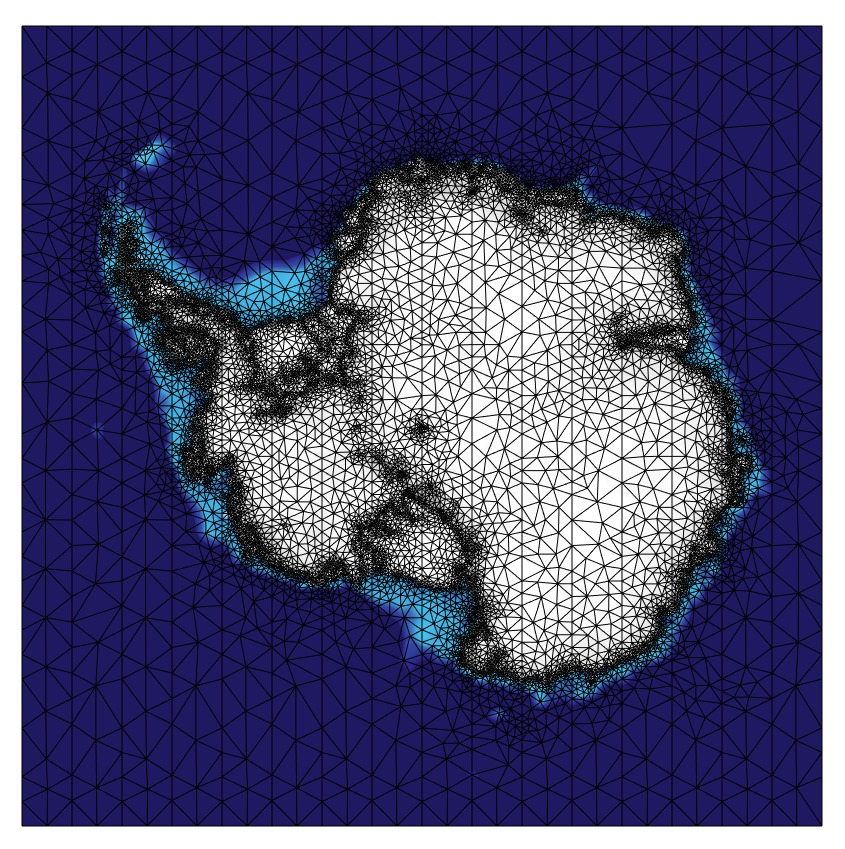
\includegraphics[width=0.8\linewidth]{Fig_UFEMISM.jpg}
  \end{figure}  

  \paragraph{Abstract}
  
The Utrecht Finite voluMe Ice-Sheet Model (UFEMISM) is an ice-sheet-shelf model that solves the hybrid SIA/SSA ice-dynamical equations on a fully adaptive, unstructured grid. It has been developed at IMAU since 2020. While intended mainly for palaeo-applications, the model is very versatile, and can be used for future projections as well. This document contains a complete description of the model; a derivation of the underlying equations, a description of the data and code structure, descriptions of (most of) the subroutines, and results of several important benchmark experiments. In theory, this should give the user enough information to be able to freely use and adapt UFEMISM for their own research.
  
\newpage
\tableofcontents

\newpage
\pagenumbering{arabic}

\section{Introduction}

\subsection{Background}

The Institute for Marine and Atmospheric research Utrecht (IMAU) has a long, rich history of ice-sheet modelling. In the early 2000's, GRICE (GReenland ICE-sheet model) was created: an SIA-only model   for studying the evolution of the Greenland ice sheet during glacial cycles. Several years later this model was adapted for the Antarctic ice sheet, including a module that solved the SSA for floating ice shelves, thus becoming ANICE (ANtarctic ICE-sheet model). Around 2010 this was extended into the coupled model ANICE-SELEN, which included four copies of ANICE to simulate the large continental Pleistocene ice-sheets (North America, Eurasia, Greenland, and Antarctica), as well as the sea-level equation solver SELEN. In early 2021 ANICE was replaced by its spiritual successor IMAU-ICE; still a square-grid hybrid SIA/SSA model, but thoroughly cleaned up and restructured, so as to enable a new generation of PhD's and postdocs to use and develop it without having to first know all the details and peculiarities of the work of their numerous predecessors.\\
\\
In the late 00's and early 10's, several studies were published that showed that the phenomenon of grounding-line migration was much more important for large-scale ice-sheet evolution then previously thought, particularly in Antarctica. They also showed that the increasingly common hybrid SIA/SSA ice models (like ANICE and IMAU-ICE) performed poorly at capturing this phenomenon, partly due to their often coarse resolution. The first few of these studies suggested that, in order to solve the problem, a resolution of 100 m or less was required. This is completely unachievable for palaeo-ice-sheet models; they must be able to simulate tens or sometimes hundreds of thousands of years, which is why researchers typically use resolutions of 10 - 40 km. However, several later studies developed clever ''heuristic'' solutions to this problem, which allowed them to use much coarser resolutions (ranging from 1 km to 20 km, depending on which study you believe) and still get good results. Aside from these numerical issues with resolution, it also became clear that small-scale topographical features like fjords and underwater hills could significantly affect large-scale ice-sheet dynamics, implying that even the ''heuristic'' models would still need a resolution of a few kilometres or less.\\
\\
However, while 20 km is still manageable, 10 km is already pushing the limits of what can reasonably be done with a square-grid model, and the even finer numbers required for resolving bed topography are simply not feasible for long palaeo-simulations. The obvious solution to this, in our view, was not to use a square grid. The studies that investigated the resolution problem already noted that in order to get good results, a high resolution was required only at the grounding line, not everywhere on the ice sheet. This intuitively makes sense; surface curvature (the leading term in the truncation error of any first-order discretisation scheme) is highest near the grounding line, as are the strain rates in the ice. Also, since grounded ice is thinnest and fastest there, this is where the topographical features of the underlying bedrock become most important. By creating a grid that has a high resolution only at the grounding line and nowhere else, you can ''skip'' a lot of non-essential calculations in the interior (determining velocities for essentially stagnant ice), freeing up computation time for the rest of the model. This line of reasoning led to the inception of UFEMISM: the first palaeo-ice-sheet model to use a dynamic adaptive grid.

\subsection{Objectives}

When the development of UFEMISM first began, the following objectives were set:

\begin{itemize}

\item \textbf{Dynamic adaptive grid}: a key difference between palaeo-simulations and future projections is that the changes in ice-sheet geometry are much larger in the former. Since it is not feasible to create a single mesh that has a high resolution everywhere the grounding line might be at some point in time (which would defeat the purpose of the unstructured grid!), the mesh must be able to adapt to the ice sheet.

\item \textbf{Flexibility}: a large part of palaeoglaciological research consists of inventing new features to add to ice-sheet models, just to see what they do. This is one of the main reasons why most palaeoglaciologists use simple square-grid models; not only are they fast enough for such long simulations, they're also very easy to build by hand, enabling the individual researcher to adapt the model to suit the needs of whatever project they're working on. We wanted UFEMISM to have that same flexibility.

\item \textbf{Performance}: since the whole point of creating UFEMISM was to be able to run very long simulations at a high resolution without requiring excessive amounts of computer time, good computational performance was an important goal.

\end{itemize}

The first objective, that of the dynamic adaptive grid, immediately created the biggest challenge, since no other ice-sheet model in existence has this feature. The second objective, that of flexibility, led to the decision to create a dedicated mesh-generation algorithm for UFEMISM, rather than to build upon existing external software. While there are several packages available, developed both academically and commercially, to generate meshes and solve equations (using finite elements or other methods), from the point of view of a palaeoglaciologist these are "black boxes": they work, but you won't know how, or how to make them do something else if you need them to. Since this conflicts strongly with the objective of flexibility, we decided not to rely on such external packages, but instead develop our own codes for mesh generation and PDE solving from scratch.

\subsection{Status quo}

Currently (March 2021), the following features in UFEMISM are \textbf{operational}, in development, and \textit{planned}:

\begin{itemize}

\item \textbf{Hybrid SIA/SSA ice dynamics}
\item \textbf{Adaptive mesh}
\item \textbf{Shared-memory (single node) MPI parallelisation}
\item \textbf{Simultaneous, coupled simulation of four continental ice sheets}
\item \textbf{Glacial index / inverse-$\delta^{18}O$ forcing}
\item \textbf{Matrix-method climate model}
\item \textbf{Insolation-temperature-based SMB}
\item \textbf{Basic temperature-depth-based BMB}
\item \textbf{ELRA GIA model}
\\
\item Coupling to sea-level equation model SELEN
\\
\item \textit{Multi-node MPI parallelisation}
\item \textit{Englacial tracers ($CO_2, \delta^{18}O$)}
\item \textit{Improved thermodynamics (enthalpy-based, energy-conserving)}
\item \textit{Basal hydrology}
\item \textit{Eigencalving, cliff failure, shelf crevasse failure}
\item \textit{Improved SMB and BMB parameterisations}

\end{itemize}

Currently (March 2021), a simulation of all four ice sheets over the entire last glacial cycle (120 kyr) with a grounding line resolution of 10 km takes about 40 wall clock hours.

\newpage
\section{Model structure}

UFEMISM is intended mainly for simulations of glacial cycles. For this reason, it has the ability to simultaneously simulate the evolution of ice sheets in Greenland and Antarctica, as well as North America and Eurasia (where large ice sheets existed during the Pleistocene glacial cycles). It also includes an elaborate mix of modelled data and extrapolations for both climate and mass balance, as well as an ELRA GIA model (the coupling to the sea-level/GIA model SELEN is being worked on, but is currently not yet operational). UFEMISM has been designed from the start to include all these components, and the code/data structure has been created so as to make this easy to achieve.

\subsection{Coupler}

The Fortran90 program \textsc{ufemism\textunderscore program.f90} contains the coupler: the overarching routine that calls the different regional ice-sheet models, updates the global climate forcing, and calls the sea-level equation solver SELEN (in progress). This is done in a loop using the coupler time step dt\textunderscore coupling. The general structure of the coupler looks as follows:

\hrulefill
\begin{lstlisting}

PROGRAM UFEMISM_program

! Initialise the ice model regions
CALL initialise_model( [North America] )
CALL initialise_model( [Eurasia] )
CALL initialise_model( [Greenland] )
CALL initialise_model( [Antarctica] )

! Initialise the global climate forcing
CALL initialise_climate_forcing

t_coupling = t_start

DO WHILE (t_coupling < t_end)
	
	! Run each ice model region from t_coupling to t_coupling + dt_coupling
	CALL run_model( [North America] )
	CALL run_model( [Eurasia] )
	CALL run_model( [Greenland] )
	CALL run_model( [Antarctica] )
	
	! Advance the coupler time
	t_coupling = t_coupling + dt_coupling
	
	! Update the global climate forcing
	CALL update_climate_forcing
	
	! Solve the sea-level equation
	IF (time_since_last_SELEN > dt_SELEN) THEN
		CALL run_SELEN
	END IF
	
END DO

END PROGRAM UFEMISM_program

\end{lstlisting}
\hrulefill
\\
\\

Note that, since we generally want to update the global climate more often than the sea-level equation, SELEN is given its own seperate time step. Also note that model initialisation has been separated from model running, a practise that we have adopted everywhere in the model.

\subsection{Ice model}

The main ice model of UFEMISM is contained in the subroutine \textsc{run\textunderscore model} in the module \textsc{UFEMISM\textunderscore main\textunderscore module.f90}. This subroutine is called from the coupler and is provided one of the model regions as an in/output argument. When called, it will run that model region up till the next coupling moment. The general structure of the ice model looks as follow:

\hrulefill
\begin{lstlisting}

SUBROUTINE run_model( [region] )

DO WHILE (region%time <= t_end)

	IF (do_GIA) run_ELRA_model( [region] )
	CALL update_ice_thickness( [region] )
	IF (mesh fitness < threshold) update_mesh( [region] )
	IF (do_SIA) CALL update_SIA_velocities( [region] )
	IF (do_SSA) CALL update_SSA_velocities( [region] )
	IF (do_climate) CALL run_climate_model( [region] )
	IF (do_SMB) CALL run_SMB_model( [region] )
	IF (do_BMB) CALL run_BMB_model( [region] )
	IF (do_thermo) CALL run_thermodynamics( [region] )
	IF (do_output) CALL write_output( [region] )
	region%time = region%time + region%dt

END DO

END SUBROUTINE run_model

\end{lstlisting}
\hrulefill
\\
\\
An important feature of UFEMISM is the asynchronous time stepping of the different model components. All components have their own independent time step. The model time step \textsc{region\%dt} is determined in every loop to equal the difference between the current model time, and the first time one of the components requires an update. This is visualised below.

\begin{figure}[h!] \label{fig:timestep}
  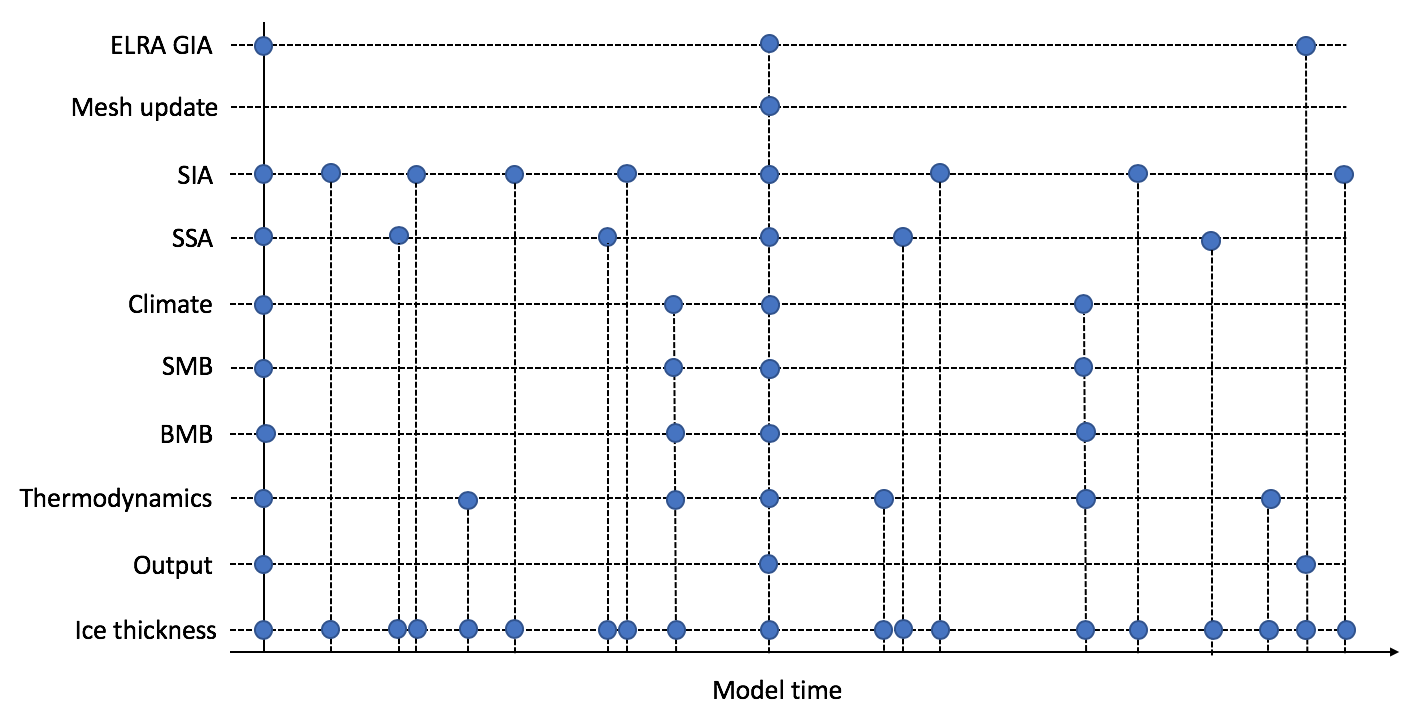
\includegraphics[width=0.9\linewidth]{Fig_timestep_UFEMISM.png}
  \caption{Asynchronous time stepping in UFEMISM.}
\end{figure}

The time steps $dt_{SIA}, dt_{SSA}$ of the SIA and SSA are calculated dynamically using their own respective stability criteria (eqs. \eqref{eq:SIA_dt} and \eqref{eq:SSA_dt}). All the other model components have fixed time steps, which are set through the config. At the end of every model loop, the subroutine \textsc{determine\textunderscore timesteps\textunderscore and\textunderscore actions} determines which model component(s) should be run next, and advances the model time to that particular moment. The mesh fitness is checked after the ice-sheet geometry has been updated. If the fitness lies below the prescribed fitness threshold, a mesh update is triggered. When this happens, only ice thickness and englacial temperature are remapped from the old to the new mesh; all other model data is calculated by running all of the model components.\\
\\
The order of the different model components is such that output written at time $t$ exactly represents the modelled ice thickness and velocity fields at that time. In order to achieve this, in the very first iteration of the first time \textsc{run\textunderscore model} is called, bedrock deformation, ice thickness, and englacial temperature are updated with a time step of zero. By the time output is written, the ice velocities, climate, SMB, and BMB are all given exactly for the initial model state at $t=0$.

\subsection{Data structure}

Data fields in UFEMISM have been organised into Fortran90 \textsc{type}s. This main advantages of this approach are that it makes the header sections of subroutines a lot smaller (since instead of passing 10 or 20 different arrays as arguments, only the type containing them needs to be passed), and that it makes it impossible to accidentally use different names for the same variables in different subroutines.\\
\\
Different data fields related to the same model component have been grouped into several \textsc{type}s called ''submodels'', such as \textsc{type\textunderscore ice\textunderscore model} for ice dynamics and \textsc{type\textunderscore smb\textunderscore model} for the surface mass balance. These submodels are grouped together into \textsc{type\textunderscore region}, which contains all the model data describing one of the four model regions. In this context, the mesh too is treated as a submodel.

\begin{itemize}
  \item \textsc{type\textunderscore region}
  \begin{itemize}
  
    \item \textsc{type\textunderscore mesh}
    \begin{itemize}
      \item \textsc{real(dp), dimension(:,:) :: V}
      \item \textsc{integer, dimension(:  ) :: nC}
      \item \textsc{integer, dimension(:,:) :: C}
      \item \textsc{integer, dimension(:  ) :: niTri}
      \item \textsc{integer, dimension(:,:) :: iTri}
      \item \ldots
    \end{itemize}
  
    \item \textsc{type\textunderscore ice\textunderscore model}
    \begin{itemize}
      \item \textsc{real(dp), dimension(:  ) :: Hi}
      \item \textsc{real(dp), dimension(:  ) :: Hb}
      \item \textsc{real(dp), dimension(:  ) :: Hs}
      \item \textsc{real(dp), dimension(:,:) :: Ti}
      \item \ldots
    \end{itemize}
    
    \item \textsc{type\textunderscore smb\textunderscore model}
    \begin{itemize}
      \item \textsc{real(dp), dimension(:,:) :: Albedo}
      \item \textsc{real(dp), dimension(:,:) :: Snowfall}
      \item \textsc{real(dp), dimension(:,:) :: Rainfall}
      \item \ldots
    \end{itemize}
    
    \item \textsc{\ldots}
      
  \end{itemize}
\end{itemize}

All these different data \textsc{type}s are defined in the \textsc{data\textunderscore types\textunderscore module}. This prevents interdependency issues, and also keeps the modules containing the subroutines clean and easy to read.\\
\\
The different submodels gathered in \textsc{type\textunderscore region} are:

\begin{itemize}
\item \textsc{mesh (type\textunderscore mesh)}: All the data particular to the mesh: the basic mesh geometry and connectivity data described in Sect. XXX, as well as all the different neighbour functions.
\item \textsc{ice (type\textunderscore ice\textunderscore model)}: All the data required to calculate ice dynamics and thermodynamics: ice thickness, bedrock elevation, surface elevation, geoid elevation, partial derivatives to $(x,y,z,t)$ of all of these, ice velocities (SIA and SSA), englacial temperature, temperature-dependent ice physical properties (thermal conductivity, heat capacity, flow factor), different masks, etc.
\item \textsc{climate (type\textunderscore climate\textunderscore model)}: All the different climate fields mapped to this regions grid, divided into ''subclimates'' containing present-day observations, GCM snapshots, and the final applied climate. This is explained in more detail in Sect. XXX.
\item \textsc{smb (type\textunderscore smb\textunderscore model)}: All the different components of the surface mass balance: snowfall, rainfall, melt, refreezing, runoff, albedo, etc.
\item \textsc{bmb (type\textunderscore bmb\textunderscore model)}: All the different components of the basal mass balance (currently only the yearly melt).
\item \textsc{pd (type\textunderscore pd\textunderscore data\textunderscore fields)}: The present-day ice-sheet geometry, used to calculate different anomalies: surface load for the GIA model, change in surface elevation for the parameterised climate, etc. This data is stored both on the current mesh, and on the original x,y-grid on which it is provided (so that, after a mesh update, it can be projected onto the updated model mesh from its original grid, to prevent numerical diffusion from accumulating).
\item \textsc{init (type\textunderscore init\textunderscore data\textunderscore fields)}: The initial ice-sheet geometry at the start of the simulation. Stored on both the mesh and the original data grid, just as the PD reference data.
\end{itemize}

\subsubsection{Shared memory}

The current version of UFEMISM has been parallelised using MPI shared memory, allowing the model to run in parallel on any number of cores that have direct access to the same memory chip. MPI uses its own routines to allocate shared memory and associate pointers with it. These have been wrapped in different routines in the \textsc{parallel\textunderscore module}:

\begin{itemize}
\item \textsc{allocate\textunderscore shared\textunderscore dp\textunderscore 0D}
\item \textsc{allocate\textunderscore shared\textunderscore bool\textunderscore 1D}
\item \textsc{allocate\textunderscore shared\textunderscore int\textunderscore 2D}
\item \ldots
\end{itemize}

The naming convention of these routines is ''\textsc{allocate\textunderscore shared\textunderscore [type]\textunderscore [dim]}''. With the exception of the \textsc{0D} variants (which allocate scalars rather than arrays), they require the dimensions to be allocated as input arguments, and return two output arguments: a \textsc{pointer} to the memory space (which is accepted by Fortran subroutines just like the array it points to), and an MPI \textsc{window} (really just an \textsc{integer}) associated with this memory space. The \textsc{window} is needed to deallocate the memory later. The subroutine \textsc{allocate\textunderscore shared\textunderscore int\textunderscore 2D} looks like this:

\hrulefill
\begin{lstlisting}

SUBROUTINE allocate_shared_int_2D( n1,n2,p,w)

! Dimension(s) of memory to be allocated
INTEGER, INTENT(IN) :: n1, n2

! Pointer to memory space
INTEGER, DIMENSION(:,:), POINTER, INTENT(OUT) :: p

! MPI window to the allocated memory space
INTEGER, INTENT(OUT) :: w

...
(allocate shared memory for the (n1-by-n2) array p
...

END SUBROUTINE allocate_shared_int_2D  

\end{lstlisting}
\hrulefill
\\
\\
The MPI windows generated by the \textsc{allocate\textunderscore shared} routines are all stored in the same \textsc{type}s that hold the variables the point to, and have the same name as the variable prefixed by the letter \textsc{w}. For example, ice thickness is stored in the type \textsc{type\textunderscore ice\textunderscore model} like:

\begin{itemize}
\item \textsc{real(dp), dimension(:), pointer :: Hi}
\item \textsc{integer :: wHi}
\end{itemize}

This shared memory can be deallocated by simply calling \textsc{deallocate\textunderscore shared}, e.g.:\\
\textsc{call deallocate\textunderscore shared( ice\%wHi)}

\subsubsection{Parallelisation}

All subroutines in UFEMISM, apart from those involved in mesh generation, are parallelised by simple domain decomposition. This is achieved by assigning to each processor a range of vertices that it is allowed to operate on. These are stored as non-shared integers $v_1,v_2$ in \textsc{type\textunderscore mesh}. For example, suppose that we wish to calculate the surface slope of the model region. This will then look something like this:

\hrulefill
\begin{lstlisting}

DO vi = mesh%v1, mesh%v2
  ice%dHs_dx( vi) = ddx( ice%Hs, vi)
END DO
CALL sync

\end{lstlisting}
\hrulefill
\\
\\

If, for example, the mesh has 1000 vertices and the model is running on 4 processors. Then the vertex ranges for the different processors will be:

\begin{table}[H]
  \begin{center}
    \begin{tabular}{l|l|l}
      \textbf{Processor} & \textbf{v1} & \textbf{v2}\\
      \hline
      0 & 1 & 250 \\
      1 & 251 & 500 \\
      2 & 501 & 750 \\ 
      3 & 751 & 1000 \\
    \end{tabular}
  \end{center}
\end{table}

These ranges are assigned during mesh generation using the \textsc{partition\textunderscore list} subroutine. Note that processors are indexed from 0; this is the MPI standard. Note also the \textsc{call sync} statement after the \textsc{DO} loop. This is simply a wrapper for the \textsc{mpi\textunderscore barrier} command, which ensures synchronisation. Although the work load of each processor is nearly the same, one of them might still be finished a little faster than the others. The \textsc{sync} statement ensures that the program is only allowed to continue once each processor has finished its work and therefore the entire data field (in this case, \textsc{ice\%dHs\textunderscore dx}) has been updated.\\
\\
This kind of parallelisation works only for ''embarassingly parallel'' problems, where operations on an element on an array do not depend on operations on any other elements. This is the case for the vast majority of calculations done in the ice model. There are a few exceptions where great care must be taken to ensure that the program will behave properly. For example, the SOR iteration in the SSA needs to stop when the smallest residual velocity across the entire mesh has decreased below the specified tolerance. This must be checked after all processes have finished updating values in their range, and the smallest value must be found for the entire mesh. Another problem that is not easily parallelised is the flood-fill algorithm that is used to determine the ocean mask; instead, this is done only by the master process, while all other processors simply wait around.\\
\\
Mesh generation is parallelised in a very different manner. This is explained in Sect. XXX.

\subsection{Output}

\subsubsection{Text files}

UFEMISM creates a number of ASCII text files containing scalar output data. These are given the prefix ''\textsc{aa\textunderscore}'' so that they will always be the first to show up in the results directory.\\
\\
The file ''\textsc{general\textunderscore output.txt}'' lists some global scalars such as global mean sea level, atmospheric CO\textsubscript{2}, deep-sea temperature, regional ice volume, contributions to the benthic $\delta^{18}O$ signal, etc.\\
\\
The regional ''\textsc{general\textunderscore output}'' files list regional scalars such as ice-sheet area, volume, volume above flotation, mean surface temperature, and the integrated mass balance components.\\
\\
The regional ''\textsc{time\textunderscore log}'' files list the computation time used by the different model components used by each region.\\
\\
Lastly, the Point-Of-Interest (POI) files list ice thickness and englacial temperature over time for the different POIs that have been specified through the config, to enable easy comparison with ice core data.

\subsubsection{NetCDF files}

Data fields are written to a number of NetCDF files. Each model region has its own set of output files, which are divided into ''\textsc{restart}'' and ''\textsc{help\textunderscore fields}'' files, and into ''\textsc{mesh}'' and ''\textsc{grid}'' files.\\
\\
\textsc{restart} files, as their name suggests, contain everything that is needed to restart a simulation (either in the event of a crash, or when it is convenient to split a long simulation into parts): ice thickness, bed topography, englacial temperature, the depth of the overlying firn layer, and the amount of melt that occurred during the previous year (used in the albedo parameterisation).\\
\\
\textsc{help\textunderscore fields} files can be configured by the user to contain a wide selection of data fields. Ice velocities (surface, basal, 3D), mass balance components (yearly or monthly), climate fields (temperature, precipitation, wind; yearly or monthly), etc. A full list of all the data fields that can be chosen can be found in the routine \textsc{create\textunderscore help\textunderscore field} in the \textsc{netcdf\textunderscore module} (where additional options can also easily be added).\\
\\
\textsc{mesh} files contain the data on the model mesh, as well as all the data describing that mesh. Since the mesh is irregularly updated during simulations, changing the number of vertices, this data cannot be contained within a single NetCDF file. Instead, whenever the mesh is updated, a new NetCDF file is created. The UFEMISM Github repository contains a number of Matlab scripts that can display mesh data.\\
\\
\textsc{grid} files contain the data on a regular square grid. The resolution of this grid can be specified through the config; UFEMISM internally generates this grid, and whenever output is written, it projects the specified model data to this grid and writes it to the grid output file. Note that here too, a distinction is made between \textsc{restart} and \textsc{help\textunderscore fields} files, but that the grid restart files cannot be used to restart the model. They are intended mainly for fast and easy output inspection, for example with NcView.

\newpage
\section{Ice dynamics and thermodynamics}

UFEMISM uses the hybrid SIA/SSA approximation to the stress balance developed by Bueler and Brown (2009). In this approach, the SIA is used to determine deformational velocities over land, while the SSA provides both deformational velocities for floating ice, and sliding velocities over land. Here, we will briefly list the equations describing these approximations.

\subsection{Shallow Ice Approximation}

The SIA assumes that all velocity gradients inside the ice sheet are negligible except for the vertical gradients of the horizontal velocities. This assumption simplifies the Navier-Stokes equation to a form that expresses the horizontal ice velocities solely in terms of local quantities (ice thickness, surface gradient, ice viscosity). This means no differential equation has to be solved numerically to obtain the velocity field, which makes it a very computationally efficient approach. The general consensus is that the SIA is accurate for the interior of an ice sheet, but cannot accurately describe ice flow near the ice margin, near the grounding line, or in other areas where the local ice thickness is no longer negligibly small compared to the horizontal length scale of the local topography.\\
\\
The SIA expresses the horizontal ice velocities $u(z),v(z)$ in the vertical column in terms of the depth-dependent ice diffusivity $D(z)$:

\begin{align} \label{eq:SIA}
D(z) &= 2 {(\rho g H)}^n {\left| \nabla H \right| }^{n-1} \int_0^z A\left( T^{\ast}(\zeta)\right) \zeta^n d\zeta \\
u(z) &= D(z) \frac{\partial h}{\partial x} \\
v(z) &= D(z) \frac{\partial h}{\partial y}
\end{align}

The depth-dependent ice diffusivity $D(z)$ is defined as a function of the ice density $\rho$, gravitational acceleration $g$, ice thickness $H$, surface gradient $\nabla h$, Glen's flow law exponent $n$, and the temperature-dependent ice flow factor $A\left( T^{\ast}(z) \right)$. For a comprehensive derivation of these equations, see e.g. Bueler and Brown (2009).\\
\\
In most ice sheet models a staggered grid is used for either the ice velocities, defining ice thickness on the regular grid, or vice versa. Early experiments with SIA ice models have shown that this approach strongly increases numerical stability, so that much larger time steps can be used. In UFEMISM this is done using the staggered mesh described in Sect. XXX. The ice thickness $H$ and the surface elevation $h$ are defined on the regular mesh, whereas the surface gradient $\nabla h$ and the ice velocities $u,v$ are defined on the staggered mesh. This also makes it very straightforward to calculate ice thickness change over time using a finite-volume approach (see Sect. XXX).\\
\\
SIA ice velocities are updated with a dynamical time step according to the CFL-criterion, which relates the largest time step that does not cause numerical instability to the (local) resolution $R$ and the SIA diffusivity $D$. For this calculation, these quantities are defined on the staggered vertices $c$:

\begin{equation} \label{eq:SIA_dt}
dt_{SIA} < \min_c \frac{R_c^2}{6D}
\end{equation}

\subsection{Shallow Shelf Approximation}

The SSA assumes that all velocity gradients inside the ice sheet are negligible except for the horizontal gradients of the horizontal velocities. This means that the gravitational driving stress is balanced by the longitunal (or ''membrane'') stresses, plus a (small) basal shear stress for ice on land. A concrete form of this stress balance is given by Bueler and Brown (2009), based on the work by MacAyeal (1989) and Weis et al. (1999):

\begin{align} \label{eq:SSA}
\frac{\partial}{\partial x} \left[ 2 \overline{\eta} H \left( 2 \frac{\partial u}{\partial x} + \frac{\partial v}{\partial y} \right) \right] +
\frac{\partial}{\partial y} \left[    \overline{\eta} H \left(    \frac{\partial u}{\partial y} + \frac{\partial v}{\partial x} \right) \right] -
\frac{\tau_c u}{|\textbf{u}|} &= \rho g H \frac{\partial h}{\partial x}, \\
\frac{\partial}{\partial y} \left[ 2 \overline{\eta} H \left( 2 \frac{\partial v}{\partial y} + \frac{\partial u}{\partial x} \right) \right] +
\frac{\partial}{\partial x} \left[    \overline{\eta} H \left(    \frac{\partial v}{\partial x} + \frac{\partial u}{\partial y} \right) \right] -
\frac{\tau_c v}{|\textbf{u}|} &= \rho g H \frac{\partial h}{\partial y}.
\end{align}

The first two terms on the left-hand sides of these equations describe the membrane stresses, in terms of the horizontal ice velocities $u,v$, the vertically averaged ice viscosity $\overline{\nu}$ and the ice thickness $H$. The last terms on the left-hand side describe the basal shear stress, related to the ice velocity through a Coulomb-type sliding law (where the magnitude of the stress is independent of the magnitude of the velocity). These stresses are balanced out by the driving stress, which is described on the right-hand sides in terms of the ice thickness $H$ and the surface slopes $h_x$ and $h_y$. The vertically averaged ice viscosity $\overline{\nu}$ is described by MacAyeal (1989) as a function of ice velocity:

\begin{equation} \label{eq:SSA_nu}
\overline{\eta} = \frac{A}{2} {\left[ 
{\left( \frac{\partial u}{\partial x} \right)}^2 + 
{\left( \frac{\partial v}{\partial y} \right)}^2 + 
\frac{\partial u}{\partial x} \frac{\partial v}{\partial y} + 
\frac14 {\left( \frac{\partial u}{\partial y} + \frac{\partial v}{\partial x} \right) }^2
\right]}^{\frac{1-n}{2n}}
\end{equation}

In UFEMISM, the SSA is further simplified following the approach by Determann (1991) and Huybrechts (1992), where the lateral variations of the effective strain rate $\frac{\partial \eta}{\partial x}, \frac{\partial \eta}{\partial y}$ are neglected. Determann (1991) and Huybrechts (1992) show that, since these terms are small compared to variations of the individual strain rates, this does not significantly affect the solution, while improving numerical stability and computational efficiency. Using this simplification, setting the basal shear stress $\tau_b = \frac{\tau_c}{|\textbf{u}|}$, and using subscript notation for partial derivatives $u_x = \frac{\partial u}{\partial x}$ simplifies to:

\begin{align} \label{eq:SSA_simple}
4 u_{xx} + u_{yy} + 3 v_{xy} - \frac{\tau_b u}{\overline{\eta}H} &= \frac{\rho g h_x}{\overline{\eta}}, \\
4 v_{yy} + v_{xx} + 3 u_{xy} - \frac{\tau_b v}{\overline{\eta}H} &= \frac{\rho g h_y}{\overline{\eta}}.
\end{align}

These equations are discretised on the mesh using the neighbour functions derived in Sect. XXX:

\begin{align} \label{eq:SSA_disc}
u^i \left( 4 N_{xx}^i + N_{yy}^i - \frac{\tau_b^i}{\overline{\eta^i} H^i} \right) + 3 v^i N_{xy}^i + 
\sum_{c=1}^n \left[ u^c \left( 4 N_{xx}^c + N_{yy}^c \right) + 3 v^c N_{xy}^c \right] &= \frac{\rho g h_x^i}{\overline{\eta^i}}, \\
v^i \left( 4 N_{yy}^i + N_{xx}^i - \frac{\tau_b^i}{\overline{\eta^i} H^i} \right) + 3 u^i N_{xy}^i + 
\sum_{c=1}^n \left[ v^c \left( 4 N_{yy}^c + N_{xx}^c \right) + 3 u^c N_{xy}^c \right] &= \frac{\rho g h_y^i}{\overline{\eta^i}}.
\end{align}

This system of linear equations can be solved using any preferred method. In UFEMISM, this is done with successive over-relaxation (SOR). This approach was chosen because the boundary conditions of the SSA (i.e. ice-sheet geometry and viscosity) tend to change very slowly over time, so that the velocity field at time $t$ is usually very similar to that at time $t+\delta t$. This means that an iterative solver using the solution from the previous time step as an initial guess will generally be more efficient than a direct solver. The choice for SOR as the particular iterative method is one of convenience, since it is very easy to implement without even having to construct a matrix representation of the system of equations.\\
\\
Let a system of linear equations be of the general form $ a_i f_i + \sum_{j \neq i} b_j f_j = c_i$. The SOR iteration scheme to find the solution $f$ then looks like:

\begin{equation}
f_i^{k+1} = f_i^k - \omega \frac{a_i f_i^k + \sum_{j \neq i} b_j f_j^k - c_i}{a_i}
\end{equation}

Applying this general form to the SSA yields the following SOR iteration scheme:

\begin{align}
u_i^{k+1} &= u_i^k - \frac{\omega}{e_{u,i}} \left( u_i^k e_{u,i} + 3 v_i^k N_{xy,i} +
\sum_{c=1}^n \left[ u_c^k \left( 4 N_{xx,c} + N_{yy,c} \right) + 3 v_c^k N_{xy,c} \right] - \frac{\rho g h_{x,i}}{\overline{\eta_i}} \right), \\
v_i^{k+1} &= v_i^k - \frac{\omega}{e_{v,i}} \left( v_i^k e_{v,i} + 3 u_i^k N_{xy,i} +
\sum_{c=1}^n \left[ v_c^k \left( 4 N_{yy,c} + N_{xx,c} \right) + 3 u_c^k N_{xy,c} \right] - \frac{\rho g h_{y,i}}{\overline{\eta_i}} \right).
\end{align}

The centre coefficients $e_{u,i}, e_{v,i}$ are defined as:

\begin{align}
e_{u,i} = 4 N_{xx,i} + N_{yy,i} - \frac{\tau_{b,i}}{\overline{\eta_i} H_i}, \\
e_{v,i} = 4 N_{yy,i} + N_{xx,i} - \frac{\tau_{b,i}}{\overline{\eta_i} H_i}.
\end{align}

Currently, no boundary conditions are applied at the calving front. Instead, following the approach by Bueler and Brown (2009), a nearly-infinitely thin (10 cm) ice shelf extends all the way to the model domain, where Neumann boundary conditions are applied. \\
\\
The over-relaxation parameter $\omega$ is currently set to $\omega = 1.1$. Higher values generally yield faster convergence, but risk numerical instability. Preliminary experiments indicate that in this case, divergence tends to occur at specific vertices, and that using a spatially variable value of $\omega$ (which is low only at these vertices and high elsewhere) can significantly decrease the number of iterations required to find an accurate solution. However, determining rules for how $\omega$ is to be defined as a function of mesh geometry such that numerical instability is guaranteed to never occur, has turned out to be difficult, and a robust implementation of this solution is left as a future project.\\
\\
SSA ice velocities are updated with a dynamical time step according to the CFL-criterion, which relates the largest time step that does not cause numerical instability to the (local) resolution $R$ and the SSA ice velocities $u,v$ $D$. For this calculation, these quantities are defined on the staggered vertices $c$:

\begin{equation} \label{eq:SSA_dt}
dt_{SSA} < \min_c \frac{R_c}{|u_c| + |v_c|}
\end{equation}

\subsection{Mass continuity}

In UFEMISM, ice thickness changes over time are calculated using a finite volume approach, which is conceptually very similar to the more commonly used combination of finite differencing with a staggered grid. Consider the conservation law for flowing ice, equating the time derivative of the ice thickness $H$ to the (two-dimensional) divergence of the ice flux (being the product of $H$ and the vertically averaged ice velocity $\textbf{u}$), and the mass balance $M$:

\begin{equation} \label{iceconsvlaw}
\frac{\partial H}{\partial t} = -\nabla \cdot \left( \mathbf{u} H \right) + M
\end{equation}

By applying the divergence theorem, this can be rewritten as:

\begin{equation}
\frac{\partial \overline{H_{\Omega}}}{\partial t} = \left[ \frac{-1}{A_{\Omega}} \oint_{\partial \Omega} \left( \mathbf{u}H \cdot d\mathbf{\hat{n}} \right) \right] + \overline{M}
\end{equation}

Here, $\Omega$ is some arbitrary 2-D region (the control “volume” after which the finite volume approach is named), enclosed by the 1-D curve $\partial \Omega$ with outward unit normal vector $\textbf{\^{n}}$ ̂. The unstructured triangular mesh partitions the 2-D domain into Voronoi cells, which function as the control volumes (see ).

\begin{figure}[h!] \label{fig:masscontinuity}
  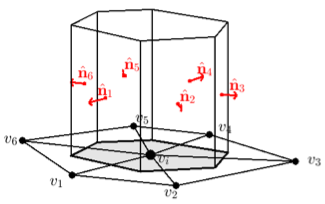
\includegraphics[width=0.3\linewidth]{Fig_masscontinuity.png}
  \caption{The Voronoi cell (grey) of a vertex serves as the control volume in the finite volume approach. Ice flows through the vertical faces of the volume, while the surface and basal mass balance add or remove ice from the top and bottom faces, respectively}
\end{figure}

The conservation law for a single Voronoi cell reads:

\begin{equation}
\frac{\partial \overline{H_i}}{\partial t} = \left[ \frac{-1}{A_i} \sum_{c=1}^n \int_{\partial_c} \left( \mathbf{u}_c H_c \cdot d\mathbf{\hat{n_c}} \right) \right] + \overline{M_i}
\end{equation}

Here, the Voronoi cell of vertex $i$ shares the boundary $\partial_c$ with that of neighbouring vertex $c$. The equation is then discretised in space by assuming that the ice velocity $\textbf{u}$ and the ice thickness $H$ are constant on $\partial_c$, so that the line integral becomes a simple multiplication with the length $L_c$ of the shared boundary $\partial_c$:

\begin{equation}
\frac{\partial \overline{H_i}}{\partial t} = \left[ \frac{-1}{A_i} \sum_{c=1}^n \left( L_c \mathbf{u}_c H_c \cdot d\mathbf{\hat{n_c}} \right) \right] + \overline{M_i}
\end{equation}

Lastly, the equation is discretised explicitly in time:

\begin{equation}
H_i^{t+\Delta t} = H_i^t + \Delta t \left( \left[ \frac{-1}{A_i} \sum_{c=1}^n \left( L_c \mathbf{u}_c H_c \cdot d\mathbf{\hat{n_c}} \right) \right] + \overline{M_i} \right)
\end{equation}

In order to solve this equation, we need to know the ice velocities $\textbf{u}_c$ on the Voronoi cell boundaries. Both the SIA and the SSA are therefore solved on the staggered vertices described earlier. The staggered ice thickness $H_c$ is determined using an up-wind scheme ($H_c=H_i$ if ice flows from $i$ to $j$, $H_c=H_j$ if it flows from$ $j to $i$). This means that the finite volume approach is essentially identical to the ''mass-conserving up-wind finite difference scheme'' used in PISM (Winkelmann et al., 2011), and very similar to the combination of finite differences with a staggered grid used in many other ice-sheet models.\\
\\
A simple flux-correction scheme is applied to prevent negative ice thicknesses from occurring. After the fluxes across all Voronoi cell boundaries have been calculated, a check is done to find vertices where $H_i^{t+\Delta t}<0$. There, all outgoing fluxes are reduced by a scaling factor so that $H_i^{t+\Delta t}=0$. Since this rescaling is applied to the staggered fluxes before the final ice thickness update is applied, this scheme is still mass-conserving.

\subsection{Thermodynamics}

UFEMISM uses the approach developed for SICOPOLIS (Greve et al., 1997) to solve the heat equation in a flowing medium:

\begin{equation}
\frac{\partial T}{\partial t} = \frac{k}{\rho c_p} \nabla^2 T - \mathbf{u} \cdot \nabla T + \frac{\Phi}{\rho c_p}.
\end{equation}

Here, the first term $\frac{k}{\rho c_p} \nabla^2 T$ represents diffusion, the second term $\mathbf{u} \cdot \nabla T$ represent advection, and the third term $\frac{\Phi}{\rho c_p}$ represents internal heating. For ice on land, internal heating is related to the vertical shear strain rates:

\begin{equation}
\Phi = 2 \left( \dot{\epsilon_{xz}} \tau_{xz} + \dot{\epsilon_{yz}} \tau_{yz} \right).
\end{equation}

Furthermore, since the horizontal dimensions of the ice sheet are so much larger than the vertical dimension, horizontal diffusion of heat is neglected, simplifying the heat equation to:

\begin{equation}
\frac{\partial T}{\partial t} = \frac{k}{\rho c_p} \frac{\partial^2 T}{\partial z^2} - \mathbf{u} \cdot \nabla T + \frac{\Phi}{\rho c_p}.
\end{equation}

This equation is discretised on an irregular grid in the vertical direction. All vertical derivatives are discretised implicitly, whereas horizontal derivatives are discretised explicitly. This mixed approach, which was first used in the ice-sheet model SICOPOLIS (Greve, 1997), is numerically stable (since both the steepest gradients and shortest grid distances are in the vertical direction), relatively easy to implement, and fast to compute. Using 15 layers in the vertical direction, a time step of 10 years is typically sufficient to maintain numerical stability, independent of the horizontal resolution.\\
\\
In order to calculate a depth-dependent temperature distribution, a vertical spatial discretisation is required. Following the approach used by many ice-sheet models, we adopt a scaled vertical coordinate:

\begin{equation} \label{eq:zeta}
\zeta = \frac{h-z}{H}
\end{equation}

This guarantees that the top and bottom of the vertical ice column always coincide with the first and last vertical grid point, 5 respectively. This coordinate transformation results in the appearance of a few extra terms in the heat equation:

\begin{equation}
\frac{\partial T}{\partial t} + \frac{\partial T}{\partial \zeta} \frac{\partial \zeta}{\partial t} =
\frac{k}{\rho c_p} \frac{\partial^2 T}{\partial \zeta^2} {\left( \frac{\partial \zeta}{\partial z} \right) }^2
- u \left( \frac{\partial T}{\partial x} + \frac{\partial T}{\partial \zeta} \frac{\partial \zeta}{\partial x} \right)
- v \left( \frac{\partial T}{\partial y} + \frac{\partial T}{\partial \zeta} \frac{\partial \zeta}{\partial y} \right)
- w \left( \frac{\partial T}{\partial \zeta} \frac{\partial \zeta}{\partial z} \right)
+ \frac{\Phi}{\rho c_p}.
\end{equation}

The different spatial derivatives of $\zeta$ follow from \eqref{eq:zeta}:

\begin{align}
\frac{\partial \zeta}{\partial t} &= \frac{1}{H} \left( \frac{\partial h}{\partial t} - \zeta \frac{\partial H}{\partial t} \right), \\
\frac{\partial \zeta}{\partial x} &= \frac{1}{H} \left( \frac{\partial h}{\partial x} - \zeta \frac{\partial H}{\partial x} \right), \\
\frac{\partial \zeta}{\partial y} &= \frac{1}{H} \left( \frac{\partial h}{\partial y} - \zeta \frac{\partial H}{\partial y} \right), \\
\frac{\partial \zeta}{\partial z} &= \frac{-1}{H}.
\end{align}

The partial derivatives $\frac{\partial T}{\partial \zeta}, \frac{\partial^2 T}{\partial \zeta^2}$ can be discretised on the irregular vertical grid using Taylor expansions, yielding expressions of the form:

\begin{align}
\frac{\partial T^k}{\partial \zeta} &= a_{\zeta} T^{k-1} + b_{\zeta} T^k + c_{\zeta} T^{k+1}, \\
\frac{\partial^2 T^k}{\partial \zeta^2} &= a_{\zeta \zeta} T^{k-1} + b_{\zeta \zeta} T^k + c_{\zeta \zeta} T^{k+1}.
\end{align}

Note that these expressions are very similar to the neighbour functions we saw earlier. We will not include their derivation here. Using these expressions to discretise the vertical derivatives of $T$, and using an implicit time-discretisation for the vertical derivatives, yields:

\begin{equation}
\begin{split}
\frac{T_k^{t + \Delta t} - T_k^t}{\Delta t} + & \frac{\partial \zeta}{\partial t} 
\left( a_{\zeta} T_{k-1}^{t+\Delta t} + b_{\zeta} T_k^{t+\Delta t} + c_{\zeta} T_{k+1}^{t+\Delta t} \right) = \\
& \frac{k}{\rho c_p H^2} \left( a_{\zeta \zeta} T_{k-1}^{t+\Delta t} + b_{\zeta \zeta} T_k^{t+\Delta t} + c_{\zeta \zeta} T_{k+1}^{t+\Delta t} \right) \\
- & u \left[ \frac{\partial \zeta}{\partial x} \left( a_{\zeta} T_{k-1}^{t+\Delta t} + b_{\zeta} T_k^{t+\Delta t} + c_{\zeta} T_{k+1}^{t+\Delta t} \right) + \frac{\partial T}{\partial x} \right] \\
- & v \left[ \frac{\partial \zeta}{\partial y} \left( a_{\zeta} T_{k-1}^{t+\Delta t} + b_{\zeta} T_k^{t+\Delta t} + c_{\zeta} T_{k+1}^{t+\Delta t} \right) + \frac{\partial T}{\partial y} \right] \\
- & w \left[ \frac{-1}{H} \left( a_{\zeta} T_{k-1}^{t+\Delta t} + b_{\zeta} T_k^{t+\Delta t} + c_{\zeta} T_{k+1}^{t+\Delta t} \right) \right]
+ \frac{\Phi}{\rho c_p}.
\end{split}
\end{equation}

This can be rearranged to read:

\begin{equation}
\begin{split}
T_{k-1}^{t+\Delta t} & \left[ a_{\zeta} \left( \frac{\partial \zeta}{\partial t} + u \frac{\partial \zeta}{\partial x} + v \frac{\partial \zeta}{\partial y} - \frac{w}{H} \right) - \frac{a_{\zeta \zeta} k}{\rho c_p H^2} \right] \\
+ T_k^{t+\Delta t} & \left[ b_{\zeta} \left( \frac{\partial \zeta}{\partial t} + u \frac{\partial \zeta}{\partial x} + v \frac{\partial \zeta}{\partial y} - \frac{w}{H} \right) - \frac{b_{\zeta \zeta} k}{\rho c_p H^2} - \frac{1}{\Delta t} \right] \\
+ T_{k+1}^{t+\Delta t} & \left[ c_{\zeta} \left( \frac{\partial \zeta}{\partial t} + u \frac{\partial \zeta}{\partial x} + v \frac{\partial \zeta}{\partial y} - \frac{w}{H} \right) - \frac{c_{\zeta \zeta} k}{\rho c_p H^2} \right] \\
= & \frac{T_k^t}{\Delta t} - u \frac{\partial T}{\partial x} - v \frac{\partial T}{\partial y} + \frac{\Phi}{\rho c_p}.
\end{split}
\end{equation}

If the vertical direction is discretised into $n$ unevenly spaced layers, this system of equations can be represented by the matrix equation $A T^{t+\Delta t} = \delta$, where the lower diagonal $\alpha$, central diagonal $\beta$ and upper diagonal $\gamma$ of the tridiagonal $n$-by-$n$ matrix $A$ and the right-hand side vector $\delta$ are given by:

\begin{align}
\alpha &= a_{\zeta} \left( \frac{\partial \zeta}{\partial t} + u \frac{\partial \zeta}{\partial x} + v \frac{\partial \zeta}{\partial y} - \frac{w}{H} \right) - \frac{a_{\zeta \zeta} k}{\rho c_p H^2}, \\
\beta &= b_{\zeta} \left( \frac{\partial \zeta}{\partial t} + u \frac{\partial \zeta}{\partial x} + v \frac{\partial \zeta}{\partial y} - \frac{w}{H} \right) - \frac{b_{\zeta \zeta} k}{\rho c_p H^2} - \frac{1}{\Delta t}, \\
\gamma &= c_{\zeta} \left( \frac{\partial \zeta}{\partial t} + u \frac{\partial \zeta}{\partial x} + v \frac{\partial \zeta}{\partial y} - \frac{w}{H} \right) - \frac{c_{\zeta \zeta} k}{\rho c_p H^2}, \\
\delta &= \frac{T_k^t}{\Delta t} - u \frac{\partial T}{\partial x} - v \frac{\partial T}{\partial y} + \frac{\Phi}{\rho c_p}.
\end{align}

This matrix equation can be solved for every individual grid cell independently, making this an embarrassingly parallel problem. In UFEMISM, this is done with the Fortran package LAPACK; in Matlab, it can be done with the “backslash method”: T = A \textbackslash delta. We apply a Dirichlet boundary condition at the top of the column, keeping ice temperature equal to surface air temperature (limited to melting point). At the base, a Neumann boundary condition is applied, keeping the vertical temperature gradient fixed to a value dictated by the geothermal heat flux and the frictional heating from sliding. Ice temperature throughout the vertical column is limited to the depth-dependent pressure melting point (a non-energy-conserving approach).

\newpage
\section{Climate}

UFEMISM's climate model is the same as that in IMAU-ICE, which in turn is same as in its predecessor ANICE2.1. It uses the matrix method developed by Berends et al. (2018). Quoting that paper: ''A climate matrix, as defined by Pollard (2010), is a collection of output data from different steady-state GCM simulations that differ from each other in one or more key parameters or boundary conditions, such as prescribed atmospheric pCO\textsubscript{2}, orbital configuration, or ice-sheet configuration. At every point in time during the simulation, the location of the model state within this matrix is extracted from the matrix by interpolating between its constituent precalculated climate states.''\\
\\
Berends et al. (2018) developed a way to use modelled ice-sheet geometry as a spatially variable interpolant between two GCM snapshots, respectively describing the PI and the LGM (Singarayer and Valdes, 2010). The ice-albedo feedback and the orographic forcing of precipitation are parameterised by this interpolation, resulting in a modelled ice-sheet geometry at LGM that agrees better with geomorphological evidence than was the case with earlier versions of the IMAU ice-sheet models. Since temperature and precipitation (which together constitute the entirety of the ''climate'' that's needed to calculate the surface mass balance) are affected by ice-sheet geometry in different ways, two separate interpolation schemes are used for these quantities.\\

\subsection{Temperature}

The equations described here are contained in the subroutine \textsc{run\textunderscore climate\textunderscore model\textunderscore matrix\textunderscore pi\textunderscore lgm\textunderscore temperature} of the \textsc{climate\textunderscore module}.\\
\\
During the LGM, temperatures in the high latitudes of the northern hemisphere were between 10 and 15 K colder than pre-industrial, much more than the global mean cooling of 5 K. This temperature change has three main causes: a lower CO2 concentration in the atmosphere (global), a much higher albedo (regional), and a much higher surface elevation (local).\\
\\
The temperature interpolation scheme of the climate matrix is based on the absorbed insolation $I_{abs}$, which is defined as the product of insolation at the top of the atmosphere $Q_{TOA}$ with the inverse of the surface albedo $a$:

\begin{equation} \label{eq:matrix_Iabs}
I_{abs}(x,y) = \sum_{m=1}^{12} Q_{TOA} (x,y,m) \cdot (1 - a( x,y,m))
\end{equation}

The absorbed insolation is calculated for the modelled ice-sheet geometry at time $t$ using the insolation at the top of the atmosphere at that point in time, using the solution by Laskar et al. (2004). Absorbed insolation fields are also calculated for the two GCM snapshots, so that we have three fields: $I_{abs,mod}$, $I_{abs,PI}$, $I_{abs,LGM}$. For all three, the albedo $a$ is modelled with UFEMISM's own SMB model. The insolation-based weighting field $w_{ins}(x,y)$ is calculated by scaling $I_{abs,mod}$ between the two reference fields:

\begin{equation} \label{eq:matrix_wins_T2m}
w_{ins}(x,y) = \frac{I_{abs,mod}(x,y) - I_{abs,LGM}(x,y)}{I_{abs,PI}(x,y) - I_{abs,LGM}(x,y)}
\end{equation}

To account for the fact that a change in albedo will affect temperatures not only locally but also regionally, a Gaussian smoothing filter $F$ with a smoothing radius of 200 km and a region-wide average value are added to find the weighting field $w_{ice}$:

\begin{equation} \label{eq:matrix_wice_T2m}
w_{ice}(x,y) = \frac{1}{7} w_{ins}(x,y) + \frac{3}{7} F \left( w_{ins}(x,y) \right) + \frac{3}{7} \overline{w_{ins}(x,y)}
\end{equation}

NOTE: preliminary attempts at writing a proper (i.e. conservative, monotonic, efficient) smoothing algorithm on an unstructured mesh have not been successful. Instead, a fixed square grid is included for these operations. The weighting field $w_{ins}$ is mapped from the mesh to the square grid, smoothing is applied on the grid, and the smoothed field is mapped back to the mesh. The two mapping operations generate a certain amount of numerical diffusion, which fortunately is not a problem for a smoothing operation.\\
\\
Lastly, the atmospheric CO\textsubscript{2} concentration is included to yield the final weighting field $w_{tot}$:

\begin{align}
w_{CO_2} &= \frac{CO_2 - 190}{280 - 190}\\
w_{tot}(x,y) &= \frac{w_{CO_2} + w_{ice}(x,y)}{2}
\end{align}

This weighting field is then used to interpolate between the two GCM snapshots:

\begin{equation}
T_{ref,GCM}(x,y) = w_{tot} (x,y) \cdot T_{PI} (x,y) + \left( 1 - w_{tot} (x,y) \right) \cdot T_{LGM} (x,y)
\end{equation}

Since the native resolution of the GCM snapshots is much lower than that of the ice-sheet model, this interpolated temperature is still very ''smooth''. To correct for this, an elevation-based downscaling scheme is used. First, the reference orography of the GCM snapshots is interpolated with the same weighting field. Then, the GCM-derived lapse rate is derived to find the ice-sheet model temperature:

\begin{align}
h_{ref,GCM}(x,y) &= w_{tot} (x,y) \cdot h_{PI} (x,y) + \left( 1 - w_{tot} (x,y) \right) \cdot h_{LGM} (x,y)\\
T_{mod} (x,y) &= T_{ref,GCM} + \lambda_{GCM} (x,y) \cdot \left( h_{mod} (x,y) - h_{ref,GCM} (x,y) \right)
\end{align}

Rather than using a constant lapse rate (typical values range from 6 to 8 K / km), a GCM-derived, spatially variable lapse rate $\lambda_{GCM} (x,y)$ is calculated from the temperature and orography fields of the two GCM snapshots:

\begin{equation}
\lambda_{LGM} (x,y) = \frac{T_{LGM}(x,y) - \left( T_{PI} (x,y) + \Delta T_{LGM} \right) }{h_{LGM} (x,y) - h_{PI} (x,y)}
\end{equation}

The temperature offset $􏰀\Delta T_{LGM}$ is the mean difference in GCM-calculated temperature between the LGM and PI fields over the ice-free area in the respective model region (either North America or Eurasia) at the LGM. The rationale behind this approach is explained in detail by Berends et al. (2018); in short, it ensures that, during the inception phase of the glacial cycle, the ice-free parts of the continent experience an appropriate amount of cooling so that the ice-sheet can expand.\\

\subsection{Precipitation}

The equations described here are contained in the subroutine \textsc{run\textunderscore climate\textunderscore model\textunderscore matrix\textunderscore pi\textunderscore lgm\textunderscore precipitation} of the \textsc{climate\textunderscore module}.\\
\\
At present, Antarctica is the driest desert on Earth, with the interior of East Antarctica receiving barely a centimetre of precipitation per year. The two main reasons for this are the extreme cold, which strongly reduces the moisture carrying capacity of the atmosphere, and the geometry of the ice-sheet. The dome shape of the Antarctic (or indeed any) ice sheet results in relatively steep slopes at the margin. As the wind blows moist air from the sea towards the ice sheet, the air has to move up this slope. Moving upwards means the pressure and temperature decrease, reducing the moisture carrying capacity, and so most of the moisture precipitates onto the ice-sheet margin. Any air that reaches the plateau of the ice-sheet interior is very dry, and so hardly and precipitation occurs there. This ''plateau desert'' effect is also expected to have existed over the North American and Eurasian ice sheets during the LGM.\\
\\
This geometry-induced precipitation change is captured in the matrix method by using a different way to calculate the weighting field. Instead of absorbed insolation, ice thickness is used an interpolant:

\begin{equation} \label{eq:matrix_wice_precip}
w_{ice} (x,y) = \frac{H_{mod}(x,y) - H_{PI}(x,y)}{H_{LGM}(x,y) - H_{PI}(x,y)} \cdot
\left( \frac{V_{mod} - V_{PI}}{V_{LGM} - V_{PI}} \right)^2
\end{equation}

Here, $H(x,y)$ is the local ice thickness, while $V = \iint H dA$ is the total regional ice volume. Note that \eqref{eq:matrix_wice_precip} is slightly different from Eq. 12 in Berends et al. (2018); the version in the paper is wrong, in the actual model code the scaled local ice thickness is multiplied with the square of the scaled ice volume.\\
\\
The final weighting field $w_{tot}(x,y)$ is obtained by applied a Gaussian smoothing filter $F$ with a radius of 200 km:

\begin{equation}
w_{tot} (x,y) = 1 - F( w_{ice} (x,y) )
\end{equation}

Note that the weight is inverted so that a value of 1 corresponds to PI conditions.\\
\\
The GCM precipitation fields are then interpolated with this weighting field:

\begin{equation}
P_{ref,GCM} (x,y) = w_{tot} (x,y) \cdot P_{PI} (x,y) + \left( 1 - w_{tot} (x,y) \right) \cdot P_{LGM} (x,y)
\end{equation}

As with the temperature, the resulting precipitation is still very ''smooth'' because of the low GCM resolution. Here too, an orography-based downscaling scheme is used to transform the precipitation from the smooth reference orography to the ''fine'' model orography. This is done using the temperature/orography precipitation model developed by Roe and Lindzen (2001), which models precipitation as a function of surface temperature, wind speed and direction, and surface slope (parameterising both the effects of temperature on atmospheric moisture carrying capacity, and of orographic forcing of precipitation).

\begin{align}
e_{sat} &= e_0 e^{\frac{c_1 (T - T_0)}{c_2 + T - T_0}} \\
w_{vv} &= max(0, u_{wind} \frac{\partial h}{\partial x} + v_{wind} \frac{\partial h}{\partial y}) \\
f( w_{vv}') &= \frac{1}{N} e^{-{\left( \frac{w_{vv}' - w_0}{\alpha} \right)}^2}\\
dP_{RL} &= e_{sat} max(0, a+b w_{vv}') f( w_{vv}') dw_{vv}'
\end{align}

Here, $e_{sat}$ is the saturation vapour pressure at the surface, which is a good proxy for the moisture content of the overlying air column. It is described by a Clausius-Clapeyron relation using the monthly mean surface temperature $T$, where $e_0$ = 6.112 mbar, $c_1$ = 17.67, and $c_2$ = 243.5 K. The vertical wind velocity $w_{vv}$ is calculated from the 850 hPa wind $[u_{wind},v_{wind}]$and the surface gradient. The precipitation $P_{RL}$ is related to vertical wind velocity $w_{vv}$ through a probability distribution $f 􏰁(w') 􏰂dw'$ , which is the probability that $w_{vv}$ lies between $w_{vv}'$ and $w_{vv}'$ + $dw_{vv}'$. $\alpha$ = 1.15 cm s\textsuperscript{-1} is the measure of variability in the vertical wind velocity (Roe, 2002). The precipitation $dP_{RL}$ is given by Eq. XX, where the constants a = 2.5 $\cdot$ 10-11 kg\textsuperscript{-1} s\textsuperscript{2} m and b = 5.9 $\cdot$ 10\textsuperscript{-9} s\textsuperscript{3} kg were obtained by tuning to observations of Greenland (Roe, 2002). This equation is solved analytically using error functions (Roe and Lindzen, 2001), resulting in the following expression:

\begin{align}
x_0 &= \frac{a}{b} + w_{vv} \\
P_{RL} &= b e_{sat} \left[ \frac{x_0}{2} + \frac{ x_o^2 erf( a |x_0| )}{2|x_0|} + \frac{e^{-\alpha^2 x_0^2}}{2 \sqrt{\pi} \alpha}\right]
\end{align}

The Roe and Lindzen precipitation model is applied to both the ''smooth'' interpolated GCM orography $h_{ref,GCM}$ (calculated with the weighting field for precipitation, which is not the same as the interpolated orography used in the temperature scheme) and to the ''fine'' modelled orography to calculate a correction factor with which the interpolated GCM precipitation $P_{ref,GCM}$ is adjusted:

\begin{equation}
P_{mod} = P_{ref,GCM} \frac{P_{RL,mod}}{P_{RL,GCM}}
\end{equation}

\newpage
\subsection{Data structure}

The current implementation of the matrix method uses the PI and LGM climates produced by Singarayer and Valdes (2010) as GCM snapshots, plus the ERA-40 reanalysis as a present-day reference state.

\begin{figure}[h!] \label{fig:climate_ERA40}
  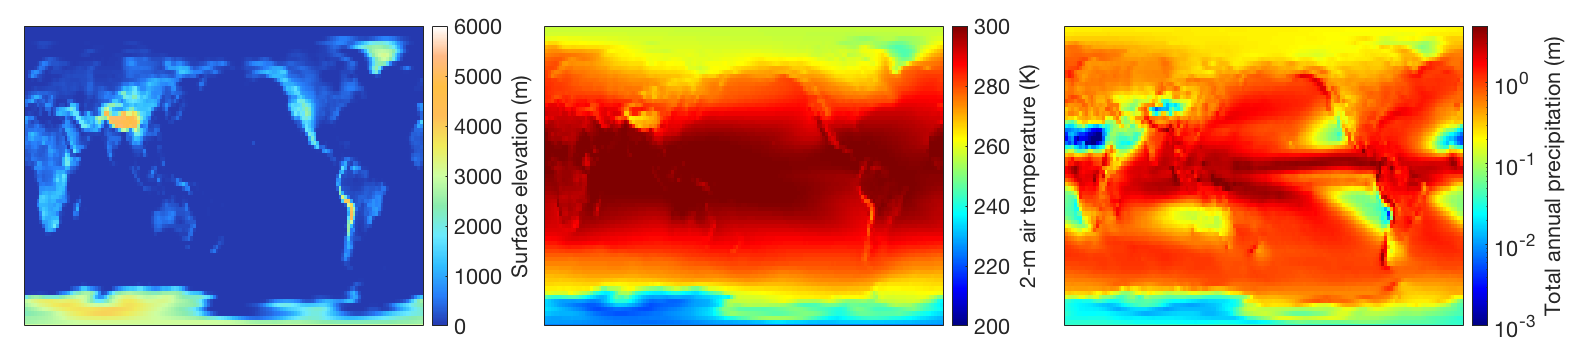
\includegraphics[width=0.95\linewidth]{Fig_climate_ERA40.png}
  \caption{The ERA-40 reanalysis data.}
\end{figure}

\begin{figure}[h!] \label{fig:climate_GCM_PI}
  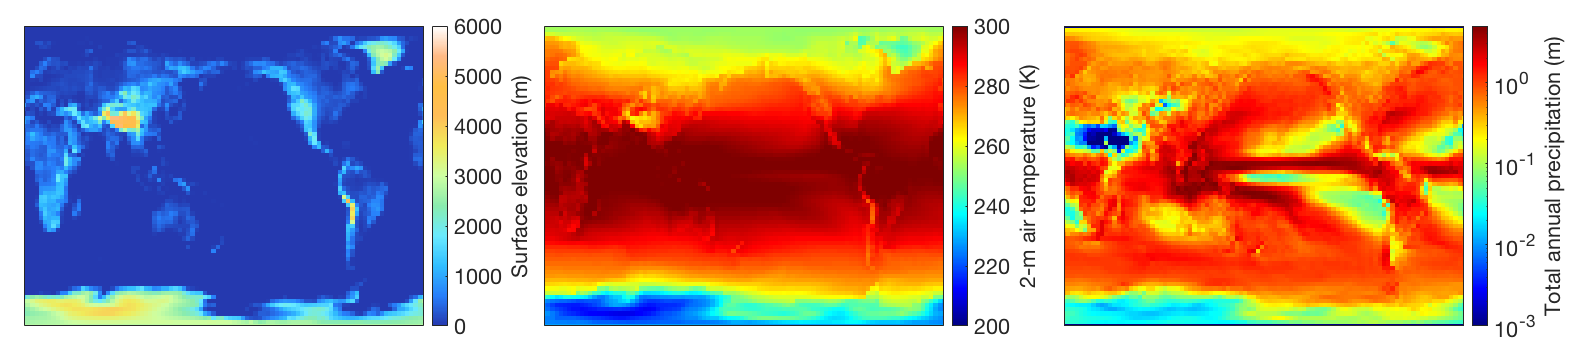
\includegraphics[width=0.95\linewidth]{Fig_climate_GCM_PI.png}
  \caption{The PI GCM snapshot by Singarayer and Valdes (2010).}
\end{figure}

\begin{figure}[h!] \label{fig:climate_GCM_LGM}
  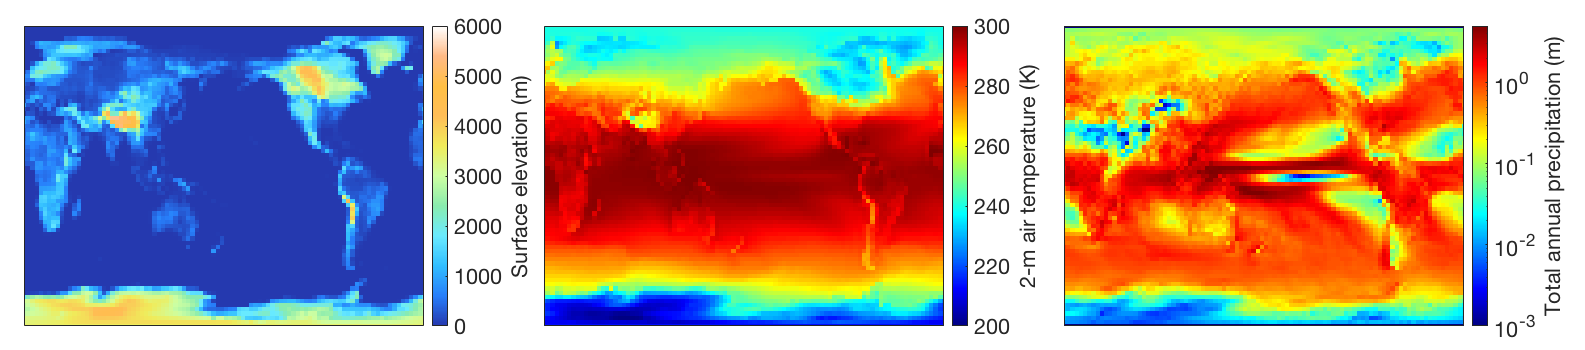
\includegraphics[width=0.95\linewidth]{Fig_climate_GCM_LGM.png}
  \caption{The LGM GCM snapshot by Singarayer and Valdes (2010).}
\end{figure}

The data structure of UFEMISM's climate model has been created specifically to accommodate the matrix method. The \textsc{type\textunderscore climate\textunderscore model} is subdivided into several ''subclimates'', which describe either the present-day observed climate \textsc{pd\textunderscore obs} (typically the ERA-40 reanalysis), the different GCM snapshot used in the matrix, or the final applied climate resulting from the matrix interpolation. This structure looks as follows:

\begin{itemize}
\item \textsc{type\textunderscore climate\textunderscore model}
\begin{itemize}

  \item \textsc{pd\textunderscore obs (type\textunderscore subclimate\textunderscore region)}
  \begin{itemize}
    \item \textsc{real(dp), dimension(:,:) :: t2m} ! Monthly mean 2-m air temperature [$K$]
    \item \textsc{real(dp), dimension(:,:) :: precip} ! Monthly total precipitation [$m$]
    \item \textsc{real(dp), dimension(:) :: Hs} ! Reference surface elevation [$m$]
    \item \textsc{real(dp), dimension(:) :: wind\textunderscore we} ! Zonal wind [$m/s$]
    \item \textsc{real(dp), dimension(:) :: wind\textunderscore sn} ! Meridional wind [$m/s$]
    \item \textsc{real(dp), dimension(:) :: wind\textunderscore lr} ! Wind in regional grid x-direction [$m/s$]
    \item \textsc{real(dp), dimension(:) :: wind\textunderscore du} ! Wind in regional grid y-direction [$m/s$]
    \item \textsc{real(dp), dimension(:) :: i\textunderscore abs} ! Yearly total absorbed insolation [$J/m^2$]
    \item \dots
  \end{itemize}
  
  \item \textsc{gcm\textunderscore pi (type\textunderscore subclimate\textunderscore region)}
  \begin{itemize}
    \item \dots
  \end{itemize}
  
  \item \textsc{gcm\textunderscore lgm (type\textunderscore subclimate\textunderscore region)}
  \begin{itemize}
    \item \dots
  \end{itemize}
  
  \item \textsc{applied (type\textunderscore subclimate\textunderscore region)}
  \begin{itemize}
    \item \dots
  \end{itemize}
  
\end{itemize}
\end{itemize}

All data fields in the \textsc{type\textunderscore climate\textunderscore model} are defined on the mesh. To easily handle mesh updates, global climates (on their respective original lat/lon grids) are stored in memory as well. These are kept in the \textsc{type\textunderscore climate\textunderscore matrix}, which is declared in \textsc{ufemism\textunderscore program} and passed to the different models as an argument. The \textsc{type\textunderscore climate\textunderscore matrix} has the same structure as the \textsc{type\textunderscore climate\textunderscore model}, with subclimates containing the present-day observed climate and the GCM snapshots. When the mesh is updated, the different subclimates are remapped from the global fields to the new mesh.

\newpage
\section{Mass balance}

The surface mass balance is modelled in UFEMISM using IMAU's in-house insolation-temperature model IMAU-ITM (Berends et al., 2018). This model took part in the GrSMBMIP intercomparison exercise (Fettweis et al., 2021), where it was shown to perform well in comparison to other parameterised SMB models when simulating the different components of the mass balance of the Greenland ice sheet during the satellite era.\\
\\
The basal melt currently consists of the temperature/depth-dependent sub-shelf melt parameterisation by Martin et al. (2011), combined with the glacial/interglacial parameterisation by Pollard and DeConto (2012), and the subtended-angle/distance-to-open-ocean parameterisation also by Pollard and DeConto (2012). Basal melt underneath grounded ice is currently not included. All of these parameterisations are currently the same as in IMAU-ICE and its predecessor ANICE2.1.

\subsection{Surface mass balance}

The surface mass balance is modelled in UFEMISM using IMAU's in-house insolation-temperature model IMAU-ITM (Berends et al., 2018; Fettweis et al., 2021). This 0-D model takes monthly values of surface temperature and precipitation, and insolation at the top of the atmosphere, to separately calculate different components of the surface mass balance.\\
\\
First, the snow fraction of precipitation is calculated according to the parameterization by Ohmura (1999), so that the  monthly precipitation $P$ is partitioned into the monthly snowfall $S$ and the monthly rainfall $R$ (all expressed in metres of water equivalent):

\begin{align}
f_{snow} &= \frac{1 - 0.796 \cdot tan^{-1} \left( \frac{T - T_0}{3.5}\right) }{2} \\
S &= P \cdot f_{snow} \\
R &= P \cdot (1 - f_{snow})
\end{align}

The monthly snowmelt $A$ is parameterised as a linear function of the 2-m air temperature $T$, the albedo $a$, and the insolation at the top of the atmosphere $Q_{TOA}$ following the approach by Bintanja et al. (2002):

\begin{equation}
A = c_1 (T - T_0) + c_2 (Q_{TOA} (1 - a)) - c_3
\end{equation}

The refreezing $F$ is calculated from the available liquid water content $L$ and the (parameterised) superimposed water content $L_{sup}$ following the approach by Huybrechts and de Wolde (1999) and Janssens and Huybrechts (2000):

\begin{align}
L &= R + A \\
L_{sup} &= 0.012 \cdot max(0, T_0 - T) \\
F &= min( L, L_{sup}, P)
\end{align}

The surface mass balance $M_s$ is equal to the sum of snowfall, (minus) ablation, and refreezing, and converted from metres of water equivalent to metres of ice equivalent:

\begin{equation}
M_s = (S - A + F) \frac{\rho_w}{\rho_i}
\end{equation}

In order to calculate the albedo used in the snowmelt parameterisation, the thickness of the firn layer $H_f$ is modelled as well, using a simple no-compaction model where any snowfall is assumed to immediately become firn with the density of ice. The firn layer thickness is limited to 10 m. The albedo $a$ is then parameterised according to the thickness of the firn layer $H_f$ and the amount of snowmelt $A_{prev}$ that occurred during the previous year:

\begin{equation}
a = a_{snow} - (a_{snow} - a_{surf}) e^{-15 H_f} - 0.015 A_{prev}
\end{equation}

Here, $a_{snow} = 0.85$ is the albedo of fresh snow, and $a_{surf}$ is the albedo of the surface underneath the firn layer (either 0.5 for bare ice, or 0.2 for bare soil).

\subsection{Basal mass balance}

The basal melt currently consists of the (linear) temperature/depth-dependent sub-shelf melt parameterisation by Martin et al. (2011), combined with the glacial/interglacial parameterisation by Pollard and DeConto (2009), and the subtended-angle/distance-to-open-ocean parameterisation also by Pollard and DeConto (2009).\\
\\
Pollard and DeConto (2009) provide a highly parameterised relation for sub-shelf melt, which depends only on horizontal shelf geometry. They provide three uniform values for sub-shelf melt underneath ''protected'', ''exposed'', and ''deep ocean'' shelves. A weighted average between these values is calculated as follows:

\begin{align}
z_e &= max[ 0, min[ 1, \frac{A - 80}{30} ]] e^{\frac{-D}{100}} \\
z_d &= max[ 0, min[ 1,  \frac{h - h_{deep}}{200} ]] \\
M &= (1 - z_d) \left[ (1 - z_e) M_p + z_e M_e \right] + z_d M_d
\end{align}

Here, the protected/exposed weighting factor $z_e$ is calculated based on the angle $A$ (degrees) subtended by the set of all straight lines from the point in question that reach open ocean without encountering land or grounded ice, and the shortest linear distance $D$ (km) from the shelf point to the open ocean. The deep-ocean weighting factor $z_d$ is calculated from the bathymetry $h$, scaled with respect to a threshold depth $h_{deep}$ which represents the transition from the continental shelf to the oceanic basin (configurable per model region).\\
\\
The three uniform melt rates for protected shelves $M_p$, exposed shelves $M_e$ and deep-ocean shelves $M_d$ are calculated as weighted averages from fixed values for the present-day, and hypothetical ''cold'' and ''warm'' ocean states. The values for these states were derived by Bas de Boer for ANICE somewhere in the early 2010' to provide reasonable patterns of Antartic advance/retreat. They are configurable per model region, with the default values copied from ANICE. The interpolation between these fixed values is done based on CO\textunderscore{2} and high-latitude insolation.\\
\\
As in ANICE and IMAU-ICE, the melt rate for protected shelves is replaced with the parameterisation by Martin et al. (2011). Here, the sub-shelf melt rate $M_p$ is parameterised as a linear function of the (mean) ocean temperature $T_{Om}$ according to Martin et al. (2011):

\begin{align}
T_{freeze} &= -1.9011 - 7.64 \cdot 10^{-4} H \frac{\rho_i}{\rho_w} \\
M_p &= \rho_w c_{pO} \gamma_T c_M \frac{T_{Om} - T_{freeze}}{L_{fus} \rho_i}
\end{align}

Here, the freezing temperature $T_{freeze}$ of ocean water at the base of the shelf is expressed as a linear function of the water depth (which is simply the ice thickness $H$ times the ratio of densities). The sub-shelf melt rate $M$ is then found from the heat capacity $C_{pO} = 3.97 \cdot 10^3 J kg^{-1} K^{-1} $ of the ocean, the thermal exchange velocity $\gamma_T = 10^{-4} m s^{-1}$, a tuning factor $c_M$ (default value 0.005), the mean ocean temperature $T_{Om}$, and the heat of fusion $L_{fus} = 3.335 \cdot 10^ J kg^{-1}$ for liquid water.\\

\newpage
\section{Glacial isostatic adjustment}

Currently, glacial isostatic adjustment (GIA) is calculated with a simple ELRA (Elastic Lithosphere, viscously Relaxed Asthenosphere) model according to Huybrechts (1992). In future improvements, the option to instead use bedrock deformation rates supplied by SELEN will be included as well.

\subsection{ELRA}

\subsubsection{Theory}

The ELRA model uses three scalar values to completely describe the response of the solid Earth to changes in loading: the flexural ridigity $D = 10^5 kg m^2 s^{-2}$ of the lithosphere, and the relaxation time $\tau = 3000 yr$ and density $\rho_m = 3300 kg m^{-3}$ of the viscous mantle (all configurable). These are used to calculate the 2D flexural profile $F$ (i.e. the equilibrium deformation in response to a unit point load), using the Kelvin function $Klv$:

\begin{align}
L_r &= {\left( \frac{D}{\rho_m g} \right) }^{\frac{1}{4}} \\
F(r) &= Klv( \frac{r}{L_r} )
\end{align}

Here, $L_r$ (m) is the influence radius of lithospheric rigidity, and $r$ is the linear distance (m) from the point load. The equilibrium bedrock deformation $\delta h_{eq}$ in response to a load distribution $P(x,y)$ is calculated by 2D convolution of the load with the flexural profile:

\begin{equation}
\delta h_{eq} (x,y) = F(r) \ast P(x,y)
\end{equation}

The lithospheric deformation rate $\frac{\partial h}{\partial t}$ is proportional to the difference between the modelled deformation :

\begin{equation}
\frac{\partial h}{\partial t} (x,y,t) = \frac{\delta h (x,y,t) - \delta h_{eq} (x,y)}{\tau}
\end{equation}

\subsubsection{Implementation}

Due to the highly diffusive nature of glacial isostatic adjustment, the ELRA model needs neither a high spatial resolution nor a small time step. Therefore, the calculation of the deformation rate $\frac{\partial h}{\partial t}$ has been given its own separate time step \textsc{dt\textunderscore elra} (configurable, default value 100 yr). Note that the bedrock elevation itself is updated in every model loop to prevent ''jumps''. Since the ELRA model does not require a high spatial resolution, and also since performing a proper 2D convolution on an unstructured mesh is not easy, the ELRA model is run on a fixed square grid (resolution configurable, default value 100 km). The surface load (relative to the present-day load, which includes both ice and liquid water) is calculated on the mesh, and then projected to this square grid. The 2D convolution is performed on the grid, and the resulting deformation rate is mapped back to the mesh. While the two mapping operations induce some small amount of numerical diffusion, this does not significantly affect the results due to the already highly diffusive nature of the ELRA model itself.\\
\\
A similar square grid construction is being developed for the coupling to SELEN.

\newpage
\section{Unstructured grid}

The core of UFEMISM is the unstructured triangular grid (the \emph{mesh}) upon which the ice-dynamical equations are discretised and solved. The data structure used
to describe the mesh (based on connectivity lists rather than matrices) has been created specifically for UFEMISM.

\subsection{Basic concepts}

Before we get started, we will briefly review some important concepts in mesh geometry.

\subsubsection{Nomenclature}

Consider the simple mesh shown in Fig. \ref{fig:dummymesh}.

\begin{figure}[h!] \label{fig:dummymesh}
  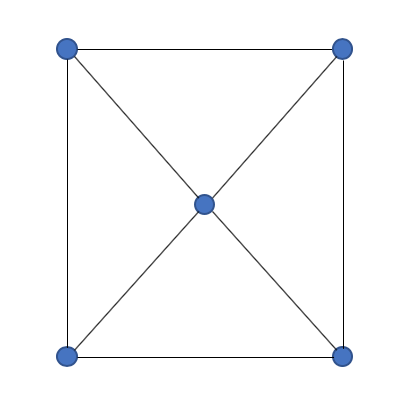
\includegraphics[width=0.3\linewidth]{Fig_dummymesh_01.png}
  \caption{A simple mesh.}
\end{figure}

This \emph{mesh} consists of five \emph{vertices}, each connected to several others by \emph{lines} and/or \emph{segments}, which together span four \emph{triangles}. Note: a connection between two vertices is called a line when the connection is a shared border of two triangles. Connections that are part of the domain boundary (and thus form the border of only a single triangle) are called segments. Vertices 1 and 2 are connected by a segment, vertices 1 and 5 are connected by a line.

\subsubsection{Voronoi cells and Delaunay triangulation}

For a given set of points in $\mathbb{R}^{2}$, a \emph{triangulation} is a way to connect the points with straight lines, such that each point is connected to at least two others by lines spanning triangles (and nothing else), without any intersecting lines. There generally exist many different triangulations for any set of points, but there is always a single unique one, called the \emph{Delaunay triangulation}, which exhibits several useful properties. Formally, the Delaunay triangulation is defined as the triangulation where the circumcircle of any triangle contains does not contain any points inside it other than the three points spanning the triangle. However, this definition is not very easy to comprehend. Instead, it is more intuitive to define the Delaunay triangulation from the concept of Voronoi cells.\\
For a given set of points in $\mathbb{R}^{2}$, each point can be assigned a region of space that is closer to that point than to any other point. This region is called the \emph{Voronoi cell} belonging to that point. The Delaunay triangulation is the triangulation where a point is connected to another point if and only if their Voronoi cells share a boundary. This is illustrated in Fig. \ref{fig:VoronoiDelaunay}.

\begin{figure}[h!] \label{fig:VoronoiDelaunay}
  \centering
  \begin{subfigure}[b]{0.25\linewidth}
    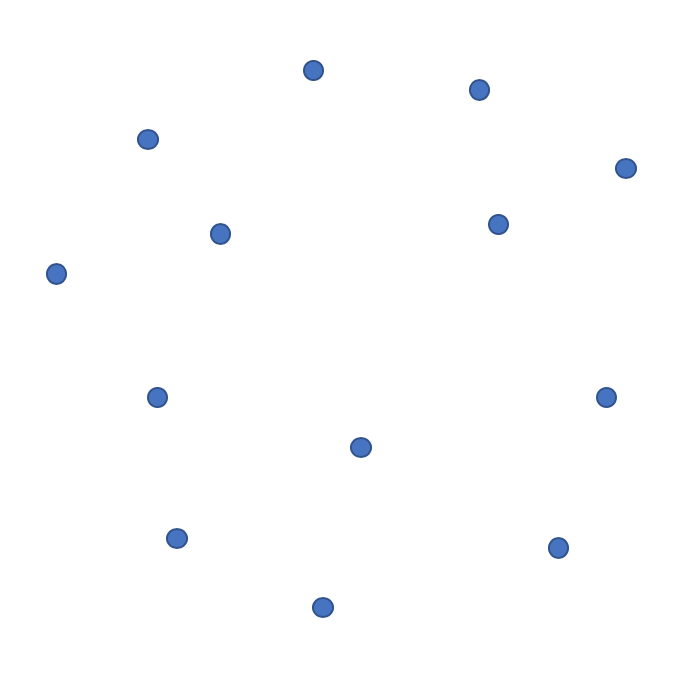
\includegraphics[width=\linewidth]{Fig_VoronoiDelaunay_01.png}
    \caption{}
  \end{subfigure}
  \begin{subfigure}[b]{0.25\linewidth}
    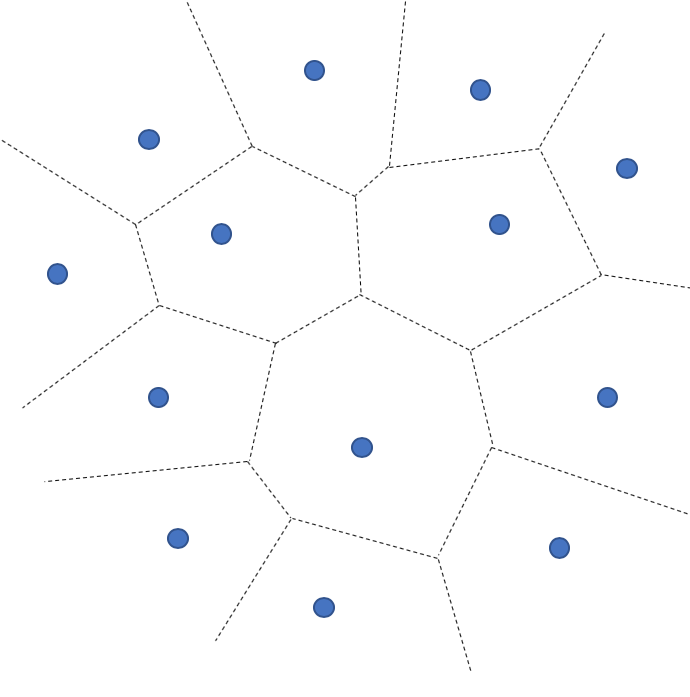
\includegraphics[width=\linewidth]{Fig_VoronoiDelaunay_02.png}
    \caption{}
  \end{subfigure}
  \begin{subfigure}[b]{0.25\linewidth}
    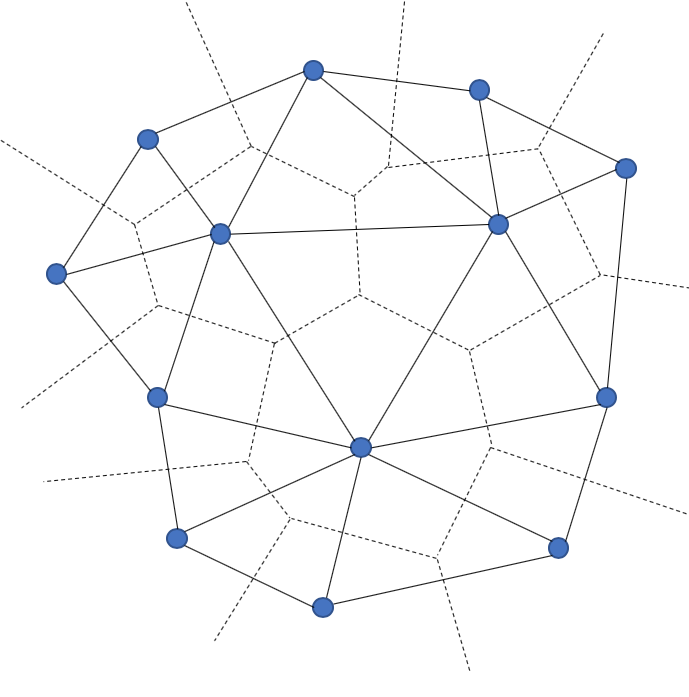
\includegraphics[width=\linewidth]{Fig_VoronoiDelaunay_03.png}
    \caption{}
  \end{subfigure}
  \caption{(a) A collection of points in $\mathbb{R}^{2}$, (b) the Voronoi cells of the points, (c) the Delaunay triangulation.}
\end{figure}

While we will not prove them, some useful properties of the Delaunay triangulation are:

\begin{itemize}
  \item The line connecting two points is always perpendicular to the shared boundary of their respective Voronoi cells.
  \item The Delaunay triangulation minimises the smallest internal angle of all triangles.
\end{itemize}

These two properties are especially useful in the context of ice-sheet models (and other fluid dynamics models). The first property is very useful when using a finite volume approach to solve the mass conservation equation, while the second one is useful for improving numerical stability. As far as I've been able to find, all models that use unstructured triangular grids use the Delaunay triangulation.\\
\\
It can be proven mathematically (if one were of a mind to do so) that any triangulation can be changed into the Delaunay triangulation by iteratively finding triangle pairs that violate the local Delaunay criterion (i.e. where the fourth vertex lies inside the circumcircle of the other three), and "flipping" them. This is illustrated in Fig. \ref{fig:Delaunayflip}.

\begin{figure}[h!] \label{fig:Delaunayflip}
  \centering
  \begin{subfigure}[b]{0.4\linewidth}
    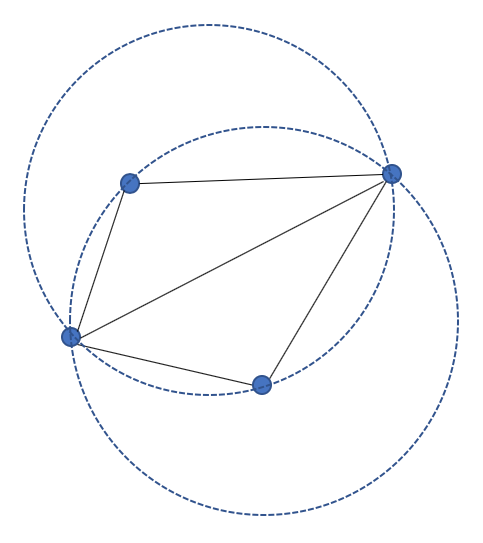
\includegraphics[width=\linewidth]{Fig_Delaunayflip_01.png}
    \caption{}
  \end{subfigure}
  \begin{subfigure}[b]{0.4\linewidth}
    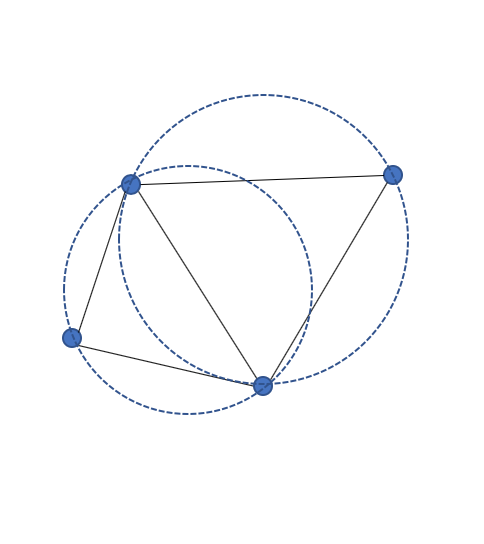
\includegraphics[width=\linewidth]{Fig_Delaunayflip_02.png}
    \caption{}
  \end{subfigure}
  \caption{(a) This pair of triangles violates the local Delaunay criterion, (b) the pair has been "flipped", and now satisfies the criterion.}
\end{figure}

\subsection{Data structure}

Theoretically, all that is needed to uniquely and completely describe a mesh is a list of the coordinates of its vertices. Everything else flows from there; their position in space determines the geometry of their Voronoi cells, which determines the Delaunay triangulation, which determines the connectivity. However, deriving all this information from the vertex coordinates can be a lengthy process, so instead several different forms of the mesh connectivity are stored in memory as well.\\
\\
A mesh consisting of \textit{nV} vertices and \textit{nTri} triangles is stored in memory in the form of vertex data and triangle data:

\begin{table}[H] \label{tab:table_vertexdatademo}
  \begin{center}
    \caption{Vertex data}
    \begin{tabular}{l|l|l}
      \textbf{Name} & \textbf{Description} & \textbf{Size}\\
      \hline
      V & Vertex [x,y] coordinates & DOUBLE(nV,2)\\
      nC & Number of connected vertices & INT(nV) \\
      C & Indices of connected vertices & INT(nV,32) \\
      niTri & Number of triangles containing this vertex & INT(nV) \\
      iTri & Indices of triangles containing this vertex & INT(nV,32) \\
      edge\textunderscore index & Edge index & INT(nV)\\
    \end{tabular}
  \end{center}
\end{table}

\begin{table}[H] \label{tab:table_triangledatademo}
  \begin{center}
    \caption{triangle data}
    \begin{tabular}{l|l|l}
      \textbf{Name} & \textbf{Description} & \textbf{Size}\\
      \hline
      Tri & Indices of the three vertices spanning this triangle & INT(nTri,3)\\
      Tricc & [x,y] coordinates of the triangle's circumcentre & DOUBLE(nTri,2) \\
      TriC & Indices of connected triangles & INT(nTri,3) \\
      Tri\textunderscore edge\textunderscore index & Edge index & INT(nTri)\\
    \end{tabular}
  \end{center}
\end{table}

As the name "unstructured mesh" suggests, there is no particular order to the indices of the vertices or triangles, and no relation between their
indices and their position. However, the following rules apply:

\begin{itemize}
  \item \textbf{C}: neighbouring vertices are listed in counterclockwise order, and only the first \textit{nC}
   entries of the 32 values per vertex are used; all other entries are zero. For vertices lying on the domain boundary, the list may not "jump" outside the domain; if, for example, this vertex lies on the eastern border, the first entry must be the neighbour lying north of the vertex on the boundary, and the last one must be the neighbour lying south of the vertex on the boundary.
  \item \textbf{iTri}: triangles containing the vertex are listed in counterclockwise order, and only the first \textit{niTri}
   entries of the 32 values per vertex are used; all other entries are zero. For boundary vertices, the same rule applies as for \textbf{C}.
  \item \textbf{Tri}: the three vertices spanning a triangle are listed in counterclockwise order. There are no rules for which vertex is listed first, but it must correspond to the entries in \textbf{TriC}.
  \item \textbf{TriC}: the three neighbouring triangles are sorted such that the first neighbouring triangles lies opposite of the first vertex, the second one across from the second vertex, etc. If no neighbouring triangle exists (i.e. when this side of the triangle is part of the domain boundary), a zero is listed.
  \item \textbf{edge\textunderscore index}: the edge index describes if a vertex lies on the domain boundary: 1 = northern boundary, 2 = north-east corner, 3 = eastern boundary, etc., 0 = not on any boundary.
  \item \textbf{Tri\textunderscore edge\textunderscore index}: similar to the edge index of vertices. The corner values (2,4,6,8) are used when a triangle is
   situated such that two if its sides lie on different parts of the domain boundary.
\end{itemize}

We will illustrate these variables with an example. Consider the simple mesh shown in Fig. \ref{fig:meshdata_02}.

\begin{figure}[H] \label{fig:meshdata_02}
  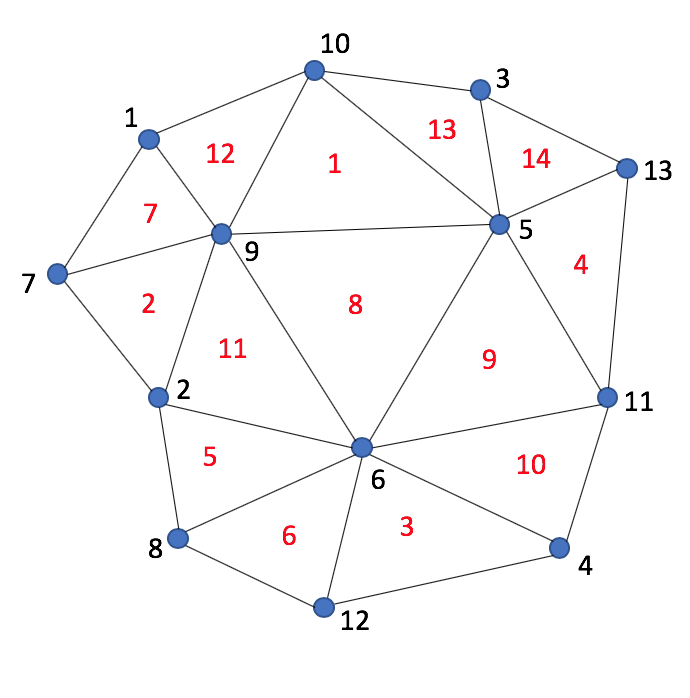
\includegraphics[width=0.5\linewidth]{Fig_meshdata_02.png}
  \caption{Another simple mesh.}
\end{figure}

The mesh data for this mesh is shown in Tables \ref{tab:table_vertexdata_01} and \ref{tab:table_triangledata_01}. Vertex coordinates \textbf{V} and triangle circumcentre coordinates \textbf{Tricc} are omitted for brevity.

\begin{table}[H] \label{tab:table_vertexdata_01}
  \begin{center}
    \caption{Vertex data}
    \begin{tabular}{l|l|l|l|l|l}
      \textbf{vi} & \textbf{V} & \textbf{nC} & \textbf{C} & \textbf{niTri} & \textbf{iTri}\\
      \hline
      1 & ... & 3 & 7,9,10 & 2 & 7,12\\
      2 & ... & 4 & 8,6,9,7 & 3 & 5,11,2\\
      3 & ... & 3 & 10,5,13 & 2 & 13,14\\
      4 & ... & 3 & 11,6,12 & 2 & 10,3\\
      5 & ... & 6 & 13,3,10,9,6,11 & 6 & 8,9,4,14,13,1\\
      6 & ... & 7 & 9,2,8,12,4,11,5 & 7 & 3,10,9,8,11,5,6\\
      7 & ... & 3 & 2,9,1 & 2 & 2,7\\
      8 & ... & 3 & 12,6,2 & 2 & 6,5\\
      9 & ... & 6 & 10,1,7,2,6,5 & 6 & 2,11,8,1,12,7\\
      10 & ... & 4 & 1,9,5,3 & 3 & 12,1,13\\
      11 & ... & 4 & 13,5,6,4 & 3 & 4,9,10\\
      12 & ... & 3 & 4,6,8 & 2 & 3,6\\
      13 & ... & 3 & 3,5,11 & 2 & 14,4\\
    \end{tabular}
  \end{center}
\end{table}

\begin{table}[H] \label{tab:table_triangledata_01}
  \begin{center}
    \caption{Triangle data}
    \begin{tabular}{l|l|l|l}
      \textbf{ti} & \textbf{Tri} & \textbf{Tricc} & \textbf{TriC}\\
      \hline
      1 & 9,5,10 & ... & 13,12,8\\
      2 & 9,7,2 & ... & 0,11,7\\
      3 & 12,4,6 & ... & 10,6,0\\
      4 & 13,5,11 & ... & 9,0,14\\
      5 & 2,8,6 & ... & 6,11,0\\
      6 & 12,6,8 & ... & 5,0,3\\
      7 & 7,9,1 & ... & 12,0,2\\\
      8 & 9,6,5 & ... & 9,1,11\\
      9 & 6,11,5 & ... & 4,8,10\\
      10 & 4,11,6 & ... & 9,3,0\\
      11 & 9,2,6 & ... & 5,8,2\\
      12 & 10,1,9 & ... & 7,1,0\\
      13 & 5,3,10 & ... & 0,1,14\\
      14 & 13,3,5 & ... & 13,4,0\\
    \end{tabular}
  \end{center}
\end{table}


\subsection{Staggered mesh}

In order to apply the finite volume method, we need to define ice fluxes on the boundaries of the Voronoi cells of the vertices. This means we need a way to efficiently keep track of these boundaries. This is done by creating a "staggered mesh", which is conceptually very similar to the Arakawa C mesh used in square-grid models.

\begin{figure}[H] \label{fig:staggeredmesh}
  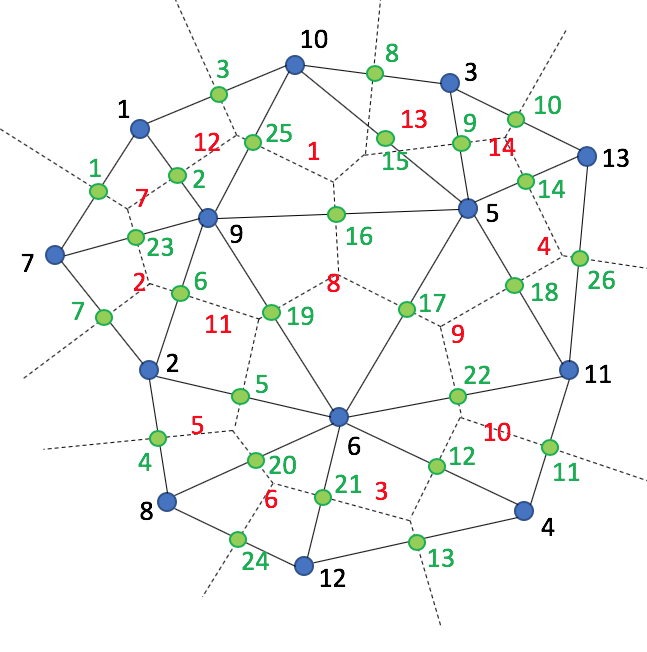
\includegraphics[width=0.5\linewidth]{Fig_staggeredmesh.png}
  \caption{The staggered vertices (green) correspond to the connections between the regular vertices (blue).}
\end{figure}

Each connection between two regular vertices is given a unique index, and represented by a staggered vertex lying halfway along the connection. Two lists are created, \textbf{Aci} and \textbf{iAci}, which relate regular vertices to staggered vertices, and vice versa. For the simple mesh shown above, these lists look like this:

\begin{table}[H] \label{tab:table_Acmesh}
  \begin{center}
    \begin{tabular}{l|l|l|l}
      \textbf{vi} & \textbf{iAci} & \textbf{ai} & \textbf{Aci}\\
      \hline
      1 & 1,2,3 & 1 & 1,7,9,0\\
      2 & 4,5,6,7 & 2 & 1,9,10,7\\
      3 & 8,9,10 & 3 & 1,10,0,9\\
      4 & 11,12,13 & 4 & 2,8,6,0\\
      5 & 14,9,15,16,17,18 & 5 & 2,6,9,8\\
      6 & 19,5,20,21,12,22,17 & 6 & 2,8,7,6\\
      7 & 7,23,1 & 7 & 2,7,0,9\\
      8 & 24,20,4 & 8 & 3,10,5,0\\
      9 & 25,2,23,6,19,16 & 9 & 3,5,13,10\\
      10 & 3,25,15,8 & 10 & 3,13,0,5\\
      11 & 26,18,22,11 & 11 & 4,11,6,0\\
      12 & 13,21,24 & 12 & 4,6,12,11\\
      13 & 10,14,26 & 13 & 4,12,0,6\\
      & & 14 & 5,13,3,11\\
      & & 15 & 5,10,9,3\\
      & & 16 & 5,9,6,10\\
      & & 17 & 5,6,11,9\\
      & & 18 & 5,11,13,6\\
      & & 19 & 6,9,2,5\\
      & & 20 & 6,8,12,2\\
      & & 21 & 6,12,4,8\\
      & & 22 & 6,11,5,4\\
      & & 23 & 7,9,1,2\\
      & & 24 & 8,12,6,0\\
      & & 25 & 9,10,1,5\\
      & & 26 & 11,13,5,0
    \end{tabular}
  \end{center}
\end{table}

\textbf{iAci} lists the staggered vertices surrounding each regular vertex. The ordering corresponds to that of \textbf{C}, so that the $j$'th staggered vertex listed for vertex $i$ lies halfway along the connection between $v_i$ and its $j$'th neighbour. \textbf{Aci} lists the regular vertices along whose connection each staggered vertex lies. Additionally, it lists the two regular vertices lying to the left and right of this connection, so that the four columns in a row of \textbf{Aci} read $[v_i,v_j,v_l,v_r]$, with $v_l$ lying to the left of the line from $v_i$ to $v_j$, and $v_r$ lying to the right. If either $v_l$ or $v_r$ does not exist (which can happen when $v_i$ and $v_j$ lie on the domain boundary), the entry is zero. Keeping track of $v_l$ and $v_r$ is very useful for calculating derivatives on the staggered vertices, as we will see in Sect. XXX on discretisation.


\subsection{Mesh refinement}

UFEMISM uses an iterative mesh refinement approach to create the model mesh. The basis for this is Ruppert's algorithm (Ruppert, 1995), which iteratively "splits" triangles (i.e. adds new vertices at their circumcentres) whose smallest internal angle lies below a certain prescribe threshold value (typically 25\degree) In pseudo-code form, this reads as follows:

\begin{tabbing}
\textbf{WHILE} \=(bad triangles exist)\\
\> Find next bad triangle\\
\> Add new vertex at this triangle's circumcentre\\
\> Update Delaunay triangulation (i.e. flip triangle pairs if needed)\\
\textbf{END WHILE}
\end{tabbing}

Ruppert (1995) proved that this algorithm converges (i.e. produces a mesh with no angles below the threshold value, no excessively small triangles, and a generally limited number of vertices) as long as the prescribed mesh boundary contains no sharp angles. Since the mesh boundary in UFEMISM is a simple rectangle, this is not a problem.\\
\\
For clarity, we will give a brief example of triangle "splitting". Consider the simple mesh shown in Fig. \ref{fig:split_triangle}. The four panels show the steps of "splitting" triangle 8 by adding a new vertex at its circumcentre, and flipping some of the newly formed triangle pairs to ensure the new mesh satisfies the Delaunay criterion.

\begin{figure}[H] \label{fig:split_triangle}
  \centering
  \begin{subfigure}[b]{0.4\linewidth}
    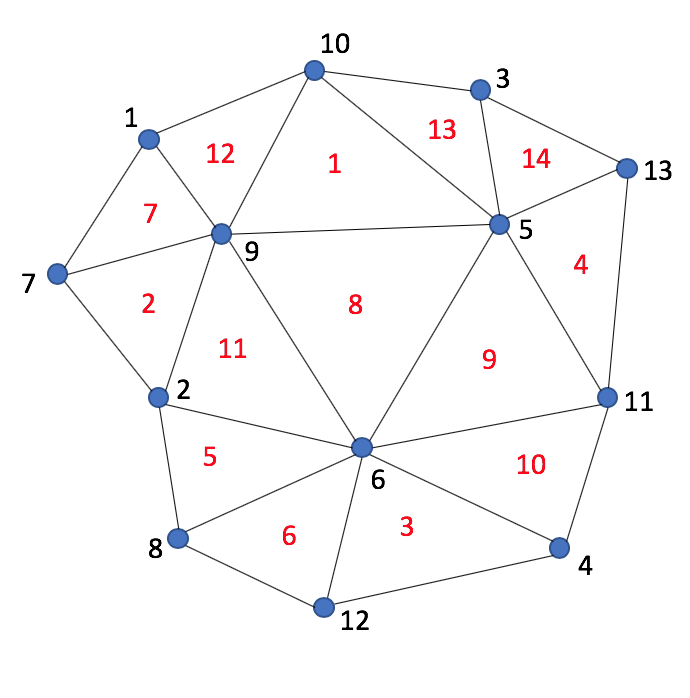
\includegraphics[width=\linewidth]{Fig_split_triangle_01.png}
    \caption{}
  \end{subfigure}
  \begin{subfigure}[b]{0.4\linewidth}
    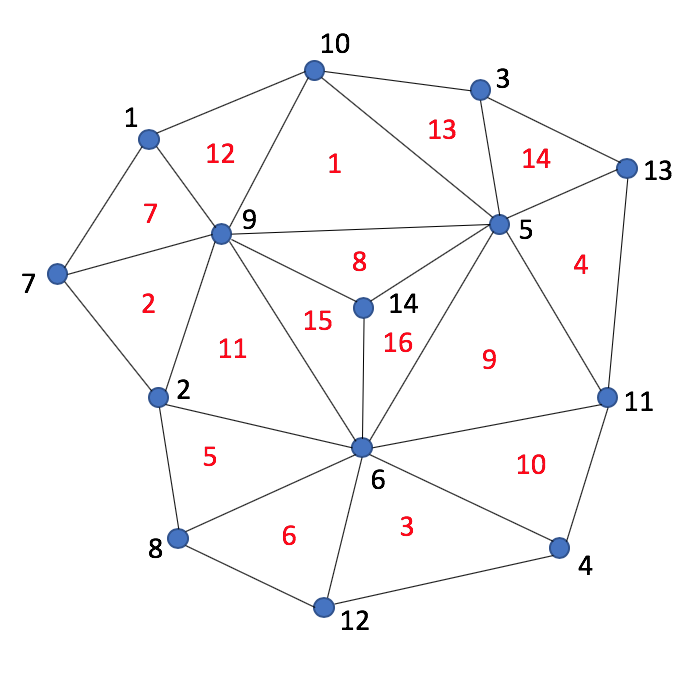
\includegraphics[width=\linewidth]{Fig_split_triangle_02.png}
    \caption{}
  \end{subfigure}
  \begin{subfigure}[b]{0.4\linewidth}
    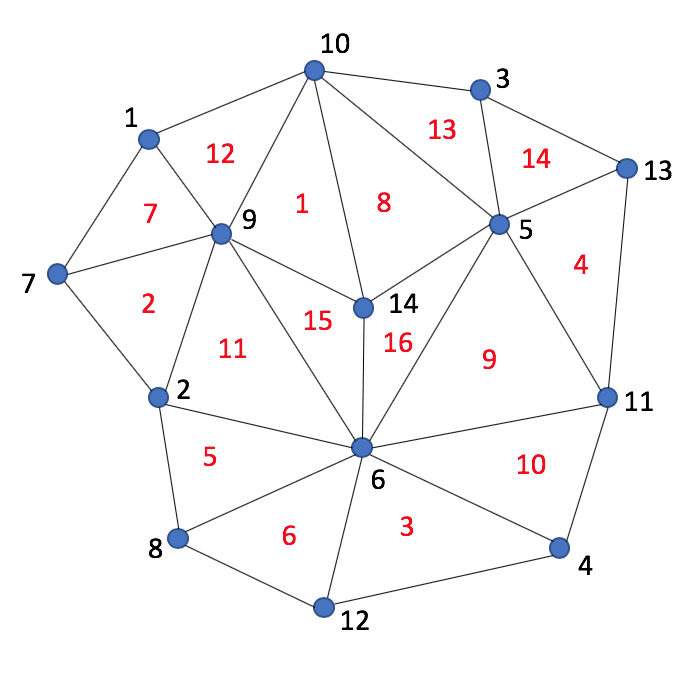
\includegraphics[width=\linewidth]{Fig_split_triangle_03.png}
    \caption{}
  \end{subfigure}
  \begin{subfigure}[b]{0.4\linewidth}
    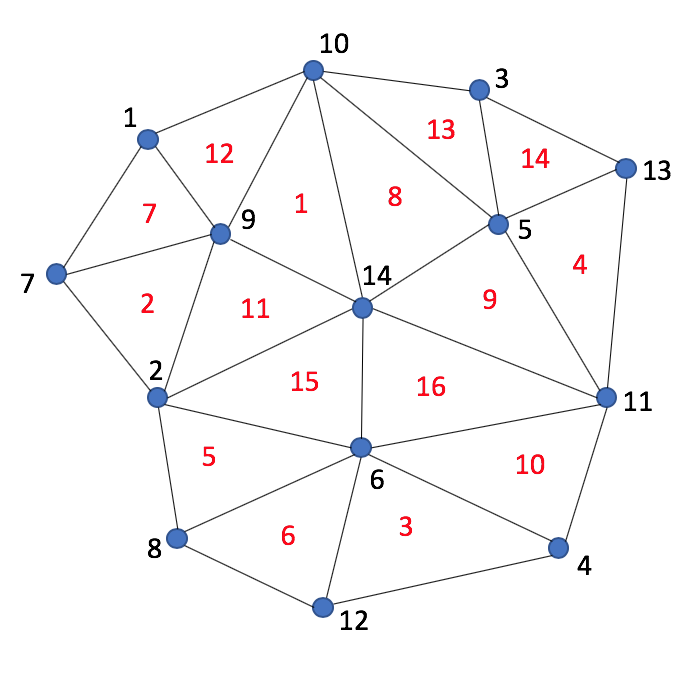
\includegraphics[width=\linewidth]{Fig_split_triangle_04.png}
    \caption{}
  \end{subfigure}
  \caption{(a) Triangle 8 is marked for splitting. (b) A new vertex is added at the circumcentre of triangle 8, replacing it by three new triangles. (c) New triangle pair 8-1 is found to violate the local Delaunay criterion, and is flipped. (d) New triangle pairs 15-11 and 16-9 were also flipped; the mesh now once again is a Delaunay triangulation.}
\end{figure}

In UFEMISM, Ruppert's algorithm has been extended to include more conditions that can cause a triangle to be marked as "bad" than just the smallest internal angle, which are based on the ice model data. Currently, the following conditions are included:

\begin{table}[H]
  \begin{center}
    \caption{mesh refinement conditions}
    \begin{tabular}{ m{10em}| m{40em} } 
      \textbf{config parameter} & \textbf{Description: triangle is marked as bad if...}\\
      \hline
      \textsc{alpha\textunderscore min} & ...any of its three internal angles is smaller than this value (original condition in Ruppert's algorithm).\\
      \textsc{res\textunderscore max} & ...any of its three sides exceeds 2 * this length.\\
      \textsc{res\textunderscore max\textunderscore gl} & ...any of its three sides exceeds 2 * this length and the grounding line passes through it.\\
      \textsc{res\textunderscore max\textunderscore cf} & ...any of its three sides exceeds 2 * this length and the calving front passes through it.\\
      \textsc{res\textunderscore max\textunderscore margin} & ...any of its three sides exceeds 2 * this length and the ice margin passes through it.\\
      \textsc{res\textunderscore max\textunderscore coast} & ...any of its three sides exceeds 2 * this length and the coastline passes through it.\\
      \textsc{poi\textunderscore resolutions} & ...any of its three sides exceeds 2 * this length and it contains a POI.\\
      \textsc{res\textunderscore max\textunderscore mountain} & ...any of its three sides exceeds $r_{crit} = 2e^{w \ln(res_{mountain}) + (1-w) \ln(res_{max})}$, with $w=\min(1,\max(0,\frac{Hb_{max} - 500}{1000}))$, where $Hb_{max}$ is the highest ice-free bedrock elevation inside the triangle.\\
    \end{tabular}
  \end{center}
\end{table}

Points of interest (POIs) are specified by their lat/lon-coordinates, and can be given individual resolutions. The \textsc{res\textunderscore max\textunderscore mountain} condition ensures a high resolution over ice-free mountains, scaling smoothly from the coarsest allowed resolution at elevations of 500 m and below, to the prescribed mountain resolution for elevations of 1500 m and above. This ensures that locations where inception can occur always have a high resolution, preventing a sudden jump in resolution when the mesh is updated from ice-free land (which typically has a resolution $res_{max}$) to ice margin.

\subsection{Paralellisation}

Mesh generation has been parallelised using a form of domain decomposition. Each processor is assigned a portion of the total model domain, and will generate a ''submesh'' for that portion only. Once this is done, the different meshes are ''merged'' to create one single mesh covering the whole model domain.

\begin{figure}[H] \label{fig:submeshes}
  \centering
  \begin{subfigure}[b]{0.1\linewidth}
    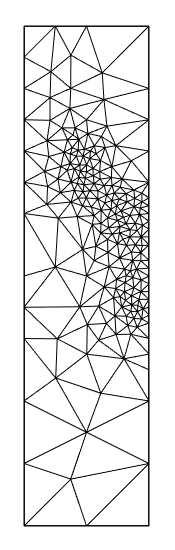
\includegraphics[width=\linewidth]{Fig_submesh1.png}
    \caption{}
  \end{subfigure}
  \begin{subfigure}[b]{0.1\linewidth}
    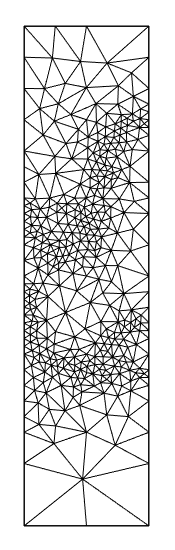
\includegraphics[width=\linewidth]{Fig_submesh2.png}
    \caption{}
  \end{subfigure}
  \begin{subfigure}[b]{0.1\linewidth}
    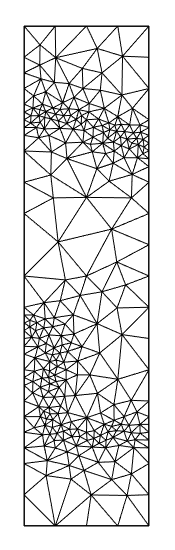
\includegraphics[width=\linewidth]{Fig_submesh3.png}
    \caption{}
  \end{subfigure}
  \begin{subfigure}[b]{0.1\linewidth}
    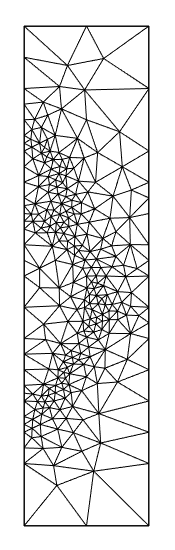
\includegraphics[width=\linewidth]{Fig_submesh4.png}
    \caption{}
  \end{subfigure}
  \caption{Four submeshes for Antarctica.}
\end{figure}

The process of mesh merging hinges on the fact that, when Rupperts algorithm refines a boundary triangle whose circumcentre lies outside the (sub)mesh domain, a new vertex is added at the midpoint of the triangle's segment. This means that boundary vertices always lie at integer sums of power-of-two fractions of a boundary edge. Looking carefully at submeshes a) and b) in the figure, we can see that many vertices on the eastern boundary of submesh a) lie at the same y-coordinate as vertices on the western boundary of submesh b). These vertices can then be merged. Generally, a small number of vertices on either boundary will have no corresponding vertex on the opposite boundary. During submesh merging, additional vertices are added first to ensure that all vertices on either boundary have corresponding vertices on the opposite boundary (a process called ''submesh alignment'').\\
\\
Since only two submeshes can be merged at a time, submesh merging is an iterative process. For example, the four submeshes in the figure would be merged in two phases. In the first phase, processor a) would be given access to the data of the submesh created by processor b). It allocates new memory that can accomodate the new (merged) submesh ab), and then merges submeshes a) and b) into this new memory. The old memory for submeshes a) and b) is then deallocated. At the same time, processor c) will do the same with submeshes c) and d), creating a new submesh cd). In the second phase, processor a) will merge submeshes ab) and cd) into the final mesh.\\
\\
The four submeshes shown above all have equal domain widths. This is generally not the case; domain widths for mesh generation are determined such that each processor will have (roughly) the same number of vertices. This is done by looking at the vertex coordinates of the previous mesh, which is assumed to be a reasonable approximation of the new mesh.

\subsection{Discretisation}

Here, we will derive a way to discretise the first and second partial derivatives of a function defined on a mesh.

\subsubsection{First-order partial derivatives}

\begin{figure}[H] \label{fig:mesh_disc_01}
  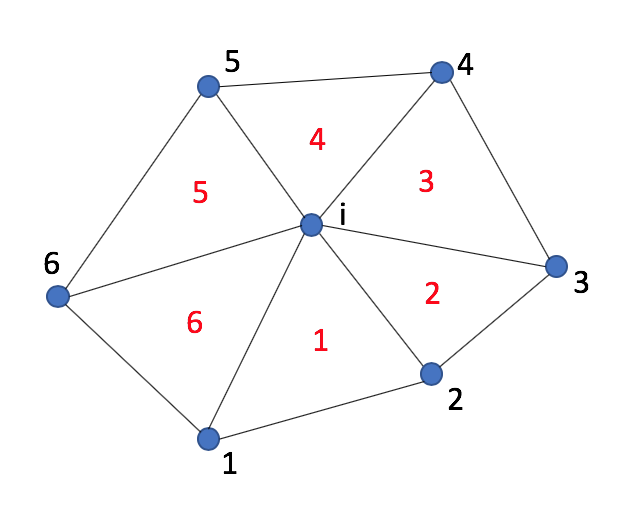
\includegraphics[width=0.3\linewidth]{Fig_mesh_disc_01.png}
  \caption{A simple mesh.}
\end{figure}

Consider the simple mesh in Fig. \ref{fig:mesh_disc_01}. Let $f$ be a function defined on the vertices of the mesh. Let vertex $i$ be connected to $n$ neighbouring vertices, thus spanning $n$ triangles (in Fig. \ref{fig:mesh_disc_01}, $n=6$). In order to derive the first partial derivatives $f_x^i$, $f_y^i$ of $f$ on vertex $i$, we will first derive the partial derivatives on the triangles surrounding $i$. Since these triangles are plane sections in $\mathbb{R}^{3}$, they have well-defined first partial derivatives, which can be expressed using the normal vector to the plane. Let vertex $i$ be described by a vector $\textbf{v}^i=\left[x^i,y^i,f^i\right]$. Triangle $t$ is then spanned by $\textbf{v}^i$, $\textbf{v}^t$ and $\textbf{v}^{t+1}$, and its normal vector is given by:

\begin{equation} \label{eq:disc_normvec}
 \textbf{n}^t = (\textbf{v}^t - \textbf{v}^i) \times (\textbf{v}^{t+1} - \textbf{v}^i) = \begin{bmatrix}
 f^i (y^{t+1} - y^t) + f^t (y^i - y^{t+1}) + f^{t+1} (y^t - y^i) \\
 f^i (x^t - x^{t+1}) + f^t (x^{t+1} - x^i) + f^{t+1} (x^i - x^t) \\ 
 (x^t - x^i) (y^{t+1} - y^i) - (y^t - y^i) (x^{t+1} - x^i)
 \end{bmatrix}.
\end{equation}

Note that indices of the "next neighbour" ($t+1$) need to be taken $mod(n)$ so that if $t=n$, then $t+1=1$.\\
\\
The first partial derivative $f_{x,tri}^t$ of $f$ on $t$ is given by:

\begin{equation} \label{eq:disc_fxtri}
f_{x,tri}^t = \frac{-n_x^t}{n_z^t}.
\end{equation}

This can be written as a linear combination of the values of $f$ on the three vertices spanning triangle $t$:

\begin{equation} \label{eq:disc_fxtri2}
f_{x,tri}^t = f^i N_{x,tri}^{t,1} + f^t N_{x,tri}^{t,2} + f^{t+1} N_{x,tri}^{t,3}.
\end{equation}

The linear coefficients $N_{x,tri}^{t,1} = \frac{y^t - y^{t+1}}{n_z^t}$, $N_{x,tri}^{t,2} = \frac{y^{t+1} - y^i}{n_z^t}$, $N_{x,tri}^{t,3} = \frac{y^t - y^i}{n_z^t}$ follow from \eqref{eq:disc_normvec} and depend only on mesh geometry, which means they only need to be calculated once. Such linear coefficients, which combine function values into a function derivative, we shall call "neighbour functions". The coefficients in \eqref{eq:disc_fxtri2} are the triangle neighbour functions for the first partial derivative on triangle $t$.\\
\\
Since the vertex $f$ represents the point where $n$ plane sections meet, the gradient of the resulting piecewise smooth surface is undefined here. We solve this by averaging the gradients of the surrounding the triangles:

\begin{equation} \label{eq:disc_fxi}
\begin{split}
f_x^i &= \frac{1}{n} \sum_{t=1}^n f_{x,tri}^t \\
 &= \frac{1}{n} \sum_{t=1}^n \left[ f^i N_{x,tri}^{t,1} + f^t N_{x,tri}^{t,2} + f^{t+1} N_{x,tri}^{t,3} \right] \\
 &= \frac{f^i}{n} \sum_{t=1}^n N_{x,tri}^{t,1} + \frac{1}{n} \sum_{t=1}^n \left[ f^t N_{x,tri}^{t,2} + f^{t+1} N_{x,tri}^{t,3} \right].
\end{split}
\end{equation}

Since the sum index $t$ is periodic in $n$ (i.e. if $t=n$ then $t+1=1$), we can use the following identity:

\begin{equation*}
\sum_{t=1}^n f^{t+1} g^t = \sum_{t=1}^n f^t g^{t-1}
\end{equation*}

This simplifies \eqref{eq:disc_fxi} to:

\begin{equation} \label{eq:disc_fxi2}
\begin{split}
f_x^i &= \frac{f^i}{n} \sum_{t=1}^n N_{x,tri}^{t,1} + \frac{1}{n} \sum_{t=1}^n \left[ f^t N_{x,tri}^{t,2} + f^{t+1} N_{x,tri}^{t,3} \right] \\
 &= \frac{f^i}{n} \sum_{t=1}^n N_{x,tri}^{t,1} + \frac{1}{n} \sum_{t=1}^n f^t ( N_{x,tri}^{t,2} + N_{x,tri}^{t-1,3} ).
\end{split}
\end{equation}

To further simplify this expression, we introduce the vertex neighbour functions $N_x^i$ for the first partial derivative on vertex $i$:

\begin{equation} \label{eq:disc_Nx}
\begin{split}
 N_x^i &= \frac{1}{n} \sum_{t=1}^n N_{x,tri}^{t,1}, \\
 N_x^t &= \frac{1}{n} ( N_{x,tri}^{t,2} + N_{x,tri}^{t-1,3} ).
\end{split}
\end{equation}

This simplifies \eqref{eq:disc_fxi2} to:

\begin{equation} \label{eq:disc_fxi3}
f_x^i = f^i N_x^i + \sum_{t=1}^n f^t N_x^t.
\end{equation}

\subsubsection{Second-order partial derivatives}

In the previous section, we expressed the first partial derivative $f_x^i$ on vertex $i$ as the average of the values on the surrounding triangles. In order to derive an expression for the second partial derivatives, we view the geometric centres of those triangles as “staggered” vertices, where the values of the first partial derivatives constitute new function values. We then construct a new set of “subtriangles”, spanned by vertex $i$ and these staggered vertices, as illustrated in Fig. A3. Since we know the values of $f_{x,tri}^t$ and $f_{y,tri}^t$ on these new vertices, we can use the same approach as before to calculate the second derivatives on the sub-triangles, and average them to get the value on vertex $i$. Preliminary experiments showed that using the geometric centre instead of the circumcentre yields more stable solutions when using these to solve differential equations. A mathematical proof of why this is the case might be interesting, but lies beyond the scope of this study.

\begin{figure}[H] \label{fig:mesh_disc_02}
  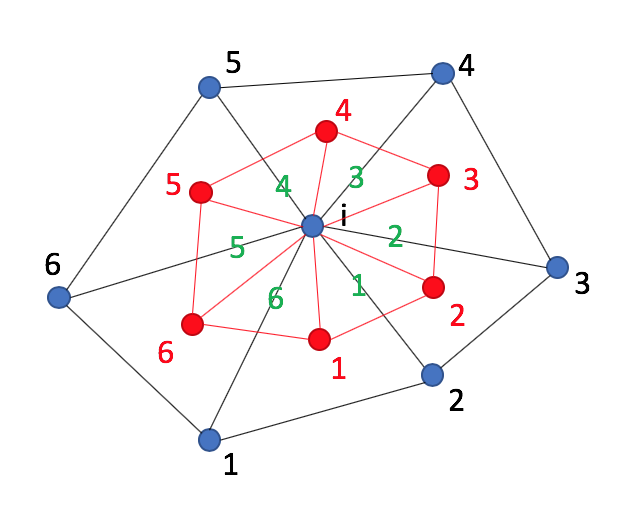
\includegraphics[width=0.3\linewidth]{Fig_mesh_disc_02.png}
  \caption{A simple mesh, with the regular vertices shown in blue. The temporary "staggered" vertices, used to derive an expression for the second partial derivatives, are shown in red. They span a new set of "subtriangles", shown in green.}
\end{figure}

A new, staggered vertex $\textbf{v}_x^t$ is created in triangle $t$, using the horizontal coordinates of the geometric centre of $t$, and the first partial derivative $f_{x,tri}^t$ of $f$ on $t$ as the vertical coordinate:

\begin{equation} \label{eq:disc_vxt}
\textbf{v}_x^t = \left[ \frac{x^i + x^t + x^{t+1}}{3}, \frac{y^i + y^t + y^{t+1}}{3}, f_{x,tri}^t \right].
\end{equation}

The subtriangle $s$ is spanned by $\textbf{v}_x^i$, $\textbf{v}_x^s$ and $\textbf{v}_x^{s+1}$, where $\textbf{v}_x^i = \left[ x^i, y^i, f_x^i \right]$, and $f_x^i$ given by \eqref{eq:disc_fxi3}. The normal vector $\textbf{n}_x^s$ to subtriangle $s$ is then given by:

\begin{equation} \label{eq:disc_normvec2}
\begin{split}
\textbf{n}_x^s &= (\textbf{v}_x^s - \textbf{v}_x^i) \times (\textbf{v}_x^{s+1} - \textbf{v}_x^i) \\
 &= \frac{1}{3} \begin{bmatrix}
 f_x^i (y^{s+2} - y^s) + f_{x,tri}^s (2y^i - y^{s+1} - y^{s+2}) + f_{x,tri}^{s+1} (y^s + y^{s+1} - y^i) \\
 f_x^i (x^s - x^{s+2}) + f_{x,tri}^s (x^{s+1} + x^{s+2} - 2x^i) + f_{x,tri}^{s+1} (2x^i - x^s - x^{s+1}) \\
 \frac{1}{3} (x^s +x^{s_1} - 2x^i) (y^{s+1} + y^{s+2} - 2y^i) - \frac{1}{3} (y^s + y^{s+1} - 2y^i) (x^{s+1} +x^{s+2} - 2x^i)
 \end{bmatrix}.
\end{split}
\end{equation}

The second partial derivatives $f_{xx,sub}^s, f_{xy,sub}^s$ of $f$ on $s$ are then given by:

\begin{equation} \label{eq:disc_fxxsub}
\begin{split}
f_{xx,sub}^s &= \frac{-n_{x,x}^s}{n_{x,z}^s}, \\
f_{xy,sub}^s &= \frac{-n_{x,y}^s}{n_{x,z}^s}.
\end{split}
\end{equation}

We then introduce the neighbour functions $N_{x,sub}^s$ for the first partial derivative on subtriangle $s$ (note that, since the function we're applying them to right now is already a first partial derivative, the result is actually a second partial derivative):

\begin{equation} \label{eq:disc_Nxsub}
\begin{split}
N_{x,sub}^s &= \frac{1}{n_{x,z}^s} \left[ (y^s - y^{s+2}), (y^{s+1} + y^{s+2} - 2y^i), (2y^i - y^s - y^{s+1}) \right], \\
N_{y,sub}^s &= \frac{1}{n_{x,z}^s} \left[ (x^{s+2} - x^s), (2x^i - x^{s+1} - x^{s+2}), (x^s + x^{s+1} - 2x^i) \right].
\end{split}
\end{equation}

This simplifies \eqref{eq:disc_fxxsub} to:

\begin{equation} \label{eq:disc_fxxsub2}
\begin{split}
f_{xx,sub}^s &= f_x^i N_{x,sub}^{s,1} + f_{x,tri}^s N_{x,sub}^{s,2} + f_{x,tri}^{s+1} N_{x,sub}^{s,3}, \\
f_{xy,sub}^s &= f_x^i N_{y,sub}^{s,1} + f_{x,tri}^s N_{y,sub}^{s,2} + f_{x,tri}^{s+1} N_{y,sub}^{s,3}. \\
\end{split}
\end{equation}

We then substitute \eqref{eq:disc_fxtri2} and \eqref{eq:disc_fxi3} into \eqref{eq:disc_fxxsub2}. From here on, only the xx-derivative is shown – xy and yy follow similar derivations:

\begin{equation} \label{eq:disc_fxxsub3}
\begin{split}
f_{xx,sub}^s &= N_{x,sub}^{s,1} \left( f^i N_x^i + \sum_{t=1}^n f^t N_x^t \right) \\
     & + N_{x,sub}^{s,2} \left( f^i N_{x,tri}^{s,1} + f^s N_{x,tri}^{s,2} + f^{s+1} N_{x,tri}^{s,3} \right) \\ 
     & + N_{x,sub}^{s,3} \left( f^i N_{x,tri}^{s+1,1} + f^{s+1} N_{x,tri}^{s+1,2} + f^{s+2} N_{x,tri}^{s+1,3} \right) \\
     &= f^i \left( N_{x,sub}^{s,1} N_x^i + N_{x,sub}^{s,2} N_{x,tri}^{s,1} + N_{x,sub}^{s,3} N_{x,tri}^{s+1,1} \right) \\
     & + f^s \left( N_{x,sub}^{s,2} N_{x,tri}^{s,2} \right) \\
     & + f^{s+1} \left( N_{x,sub}^{s,2} N_{x,tri}^{s,3} + N_{x,sub}^{s,3} N_{x,tri}^{s+1,2} \right) \\
     & + f^{s+2} \left( N_{x,sub}^{s,3} N_{x,tri}^{s+1,3} \right) \\
     & + N_{x,sub}^{s,1} \sum_{t=1}^n f^t N_x^t.
\end{split}
\end{equation}

Again, we approximate the second derivative $f_{xx}^i$ of $f$ on vertex $i$ by averaging over the surrounding subtriangles:

\begin{equation} \label{eq:disc_fxxi}
\begin{split}
f_{xx}^i &= \frac{1}{n} \sum_{s=1}^n f_{xx,sub}^s \\
     &= \frac{f^i}{n} \sum_{s=1}^n \left[ N_{x,sub}^{s,1} N_x^i + N_{x,sub}^{s,2} N_{x,tri}^{s,1} + N_{x,sub}^{s,3} N_{x,tri}^{s+1,1} \right] \\
     & + \frac{1}{n} \sum_{s=1}^n \left[ f^s \left( N_{x,sub}^{s,2} N_{x,tri}^{s,2} \right) \right] \\
     & + \frac{1}{n} \sum_{s=1}^n \left[ f^{s+1} \left( N_{x,sub}^{s,2} N_{x,tri}^{s,3} + N_{x,sub}^{s,3} N_{x,tri}^{s+1,2} \right) \right] \\
     & + \frac{1}{n} \sum_{s=1}^n \left[ f^{s+2} \left( N_{x,sub}^{s,3} N_{x,tri}^{s+1,3} \right) \right] \\
     & + \frac{1}{n} \sum_{s=1}^n \left[ N_{x,sub}^{s,1} \sum_{t=1}^n f^t N_x^t \right].
\end{split}
\end{equation}

First, we isolate the neighbour function $N_{xx}^i$  of vertex $i$ itself:

\begin{equation} \label{eq:disc_Nxxi}
N_{xx}^i = \frac{1}{n} \sum_{s=1}^n \left[ N_{x,sub}^{s,1} N_x^i + N_{x,sub}^{s,2} N_{x,tri}^{s,1} + N_{x,sub}^{s,3} N_{x,tri}^{s+1,1} \right].
\end{equation}

Then, we rearrange the sum terms containing $f^{s+1}$ by lowering the summing index by one:

\begin{equation} \label{eq:disc_fxsp1}
\begin{split}
     & \sum_{s=1}^n \left[ f^{s+1} \left( N_{x,sub}^{s,2} N_{x,tri}^{s,3} + N_{x,sub}^{s,3} N_{x,tri}^{s+1,2} \right) \right] \\
     = & \sum_{s=1}^n \left[ f^s \left( N_{x,sub}^{s-1,2} N_{x,tri}^{s-1,3} + N_{x,sub}^{s-1,3} N_{x,tri}^{s,2} \right) \right].
\end{split}
\end{equation}

We do the same for the term containing $f^{s+2}$:

\begin{equation} \label{eq:disc_fxsp2}
\begin{split}
     & \sum_{s=1}^n \left[ f^{s+2} \left( N_{x,sub}^{s,3} N_{x,tri}^{s+1,3} \right) \right] \\
     = & \sum_{s=1}^n \left[ f^s \left( N_{x,sub}^{s-2,3} N_{x,tri}^{s-1,3} \right) \right].
\end{split}
\end{equation}

Then, by observing that the inner sum in the last term in \eqref{eq:disc_fxxi} does not depend on the index of the outer sum, we rearrange this term to:

\begin{equation} \label{eq:disc_Nxxs_sum}
\sum_{s=1}^n \left[ N_{x,sub}^{s,1} \sum_{t=1}^n f^t N_x^t \right] = \sum_{s=1}^n \left[ f^s N_x^s \sum_{t=1}^n N_{x,sub}^{t,1} \right].
\end{equation}

Substituting \eqref{eq:disc_Nxxi}, \eqref{eq:disc_fxsp1}, \eqref{eq:disc_fxsp2} and \eqref{eq:disc_Nxxs_sum} into \eqref{eq:disc_fxxi} yields:

\begin{align} \label{eq:disc_fxxi2}
\begin{split}
f_{xx}^i &= f^i N_{xx}^i + \sum_{s=1}^n \left[ \frac{f^s}{n} \left( N_{x,sub}^{s,2} N_{x,tri}^{s,2} + N_{x,sub}^{s-1,2} N_{x,tri}^{s-1,3} \right. \right. \\
 & \left. \left. + N_{x,sub}^{s-1,3} N_{x,tri}^{s,2} + N_{x,sub}^{s-2,3} N_{x,tri}^{s-1,3} + N_x^s \sum_{t=1}^n N_{x,sub}^{t,1} \right) \right] \\
& = f^i N_{xx}^i + \sum_{s=1}^n \left[ \frac{f^s}{n} \left( N_{x,tri}^{s,2} \left( N_{x,sub}^{s,2} + N_{x,sub}^{s-1,3} \right) \right. \right. \\
 & \left. \left. + N_{x,tri}^{s-1,3} \left( N_{x,sub}^{s-1,2} + N_{x,sub}^{s-2,3} \right) + N_x^s \sum_{t=1}^n N_{x,sub}^{t,1} \right) \right].
\end{split}
\end{align}

As we see, this simplifies into the same form as \eqref{eq:disc_fxi3}:

\begin{equation} \label{eq:disc_fxxi3}
f_{xx}^i = f^i N_{xx}^i + \sum_{s=1}^n f^s N_{xx}^s.
\end{equation}

The neighbour functions for the second partial derivative $f_{xx}^i$ (and, following the same derivation, $f_{xy}^i$ and $f_{yy}^i$) of $f$ on vertex $i$ are therefore given by:

\begin{align} \label{eq:disc_Nxxi2}
N_{xx}^i &= \frac{1}{n} \sum_{s=1}^n \left[ N_{x,sub}^{s,1} N_x^i + N_{x,sub}^{s,2} N_{x,tri}^{s,1} + N_{x,sub}^{s,3} N_{x,tri}^{s+1,1} \right], \\
N_{xy}^i &= \frac{1}{n} \sum_{s=1}^n \left[ N_{y,sub}^{s,1} N_x^i + N_{y,sub}^{s,2} N_{x,tri}^{s,1} + N_{y,sub}^{s,3} N_{x,tri}^{s+1,1} \right], \\
N_{yy}^i &= \frac{1}{n} \sum_{s=1}^n \left[ N_{y,sub}^{s,1} N_y^i + N_{y,sub}^{s,2} N_{y,tri}^{s,1} + N_{y,sub}^{s,3} N_{y,tri}^{s+1,1} \right], \\
\begin{split} N_{xx}^s &= \frac{1}{n} \left( N_{x,tri}^{s,2} \left( N_{x,sub}^{s,2} + N_{x,sub}^{s-1,3} \right) \right. \\
 & \left. + N_{x,tri}^{s-1,3} \left( N_{x,sub}^{s-1,2} + N_{x,sub}^{s-2,3} \right) + N_x^s \sum_{t=1}^n N_{x,sub}^{t,1} \right) \end{split}, \\
\begin{split} N_{xy}^s &= \frac{1}{n} \left( N_{x,tri}^{s,2} \left( N_{y,sub}^{s,2} + N_{y,sub}^{s-1,3} \right) \right. \\
 & \left. + N_{x,tri}^{s-1,3} \left( N_{y,sub}^{s-1,2} + N_{y,sub}^{s-2,3} \right) + N_x^s \sum_{t=1}^n N_{y,sub}^{t,1} \right) \end{split}, \\
\begin{split} N_{yy}^s &= \frac{1}{n} \left( N_{y,tri}^{s,2} \left( N_{y,sub}^{s,2} + N_{y,sub}^{s-1,3} \right) \right. \\
 & \left. + N_{y,tri}^{s-1,3} \left( N_{y,sub}^{s-1,2} + N_{y,sub}^{s-2,3} \right) + N_y^s \sum_{t=1}^n N_{y,sub}^{t,1} \right) \end{split}.
\end{align}

\subsubsection{First-order derivatives on staggered vertices}

In order to solve the SIA, we require a way to discretise the first-order partial derivatives of a function on the staggered vertices described in Sect. XXX. While it is possible to just take the average value of the derivatives on the vertices themselves, as defined by \eqref{eq:disc_fxi3}, the resulting value would be a linear combination of the function values on all the neighbours of these two vertices, resulting in an undesirable degree of numerical diffusion.

\begin{figure}[H] \label{fig:mesh_staggeredvertex}
  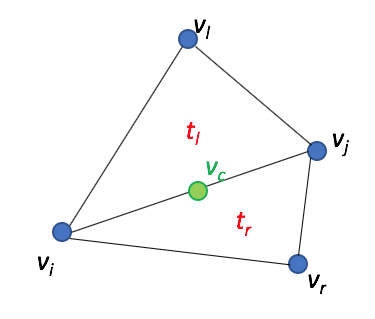
\includegraphics[width=0.3\linewidth]{Fig_staggeredvertex.png}
  \caption{A very simple mesh, showing the staggered vertex $v_c$ (green) connecting regular vertices $v_i$ and $v_j$.}
\end{figure}

Consider the simple mesh in Fig. \ref{fig:mesh_staggeredvertex}, consisting of four vertices spanning two triangles. On the two adjacent triangles $t_l$ and $t_r$, the first-order partial derivatives $f_x^l$, $f_y^l$, $f_x^r$ and $f_y^r$ are well-defined:

\begin{align} \label{eq:disc_fxlfyl}
f_x^l &= \frac{ -n_x^l }{ n_z^l } = \frac{ f^i (y^j - y^l) + f^j (y^l - y^i) + f^l (y^i - y^j)}{ x^i (y^j - y^l) + x^j (y^l - y^i) + x^l (y^i - y^j) }, \\
f_y^l &= \frac{ -n_y^l }{ n_z^l } = \frac{ f^i (x^l - x^j) + f^j (x^i - x^l) + f^l (x^j - x^i)}{ x^i (y^j - y^l) + x^j (y^l - y^i) + x^l (y^i - y^j) }, \\
f_x^r &= \frac{ -n_x^r }{ n_z^r } = \frac{ f^i (y^r - y^j) + f^j (y^i - y^r) + f^r (y^j - y^i)}{ x^i (y^r - y^j) + x^j (y^i - y^r) + x^r (y^j - y^i) }, \\
f_y^r &= \frac{ -n_y^r }{ n_z^r } = \frac{ f^i (x^j - x^r) + f^j (x^r - x^i) + f^r (x^i - x^j)}{ x^i (y^r - y^j) + x^j (y^i - y^r) + x^r (y^j - y^i) }.
\end{align}

As before, we define the derivative $f_x^c$ of $f$ on $v_c$ as the average of the values on the two adjacent triangles:

\begin{align} \label{eq:disc_fxcfyc}
f_x^c &= \frac12 (f_x^l + f_x^r), \\
f_y^c &= \frac12 (f_y^l + f_y^r).
\end{align}

The purpose of the staggered mesh is to separate velocities on cell boundaries into components parallel and orthogonal to those boundaries. The component orthogonal to the boundary carries a flux from one cell into another, while the parallel component does not. On the mesh, this is complicated by the fact that the orientation of boundaries is not fixed. Let $\textbf{u}$ be the vector pointing from $v_i$ to $v_j$:

\begin{equation} \label{eq:disc_U}
\textbf{u} = \begin{bmatrix} x_j - x_i \\ y_j - y_i \end{bmatrix}
\end{equation}

The parallel and orthogonal derivatives $f_{par}^c$ and $f_{ort}^c$ of $f$ on $v_c$ are then given by:

\begin{align} \label{eq:disc_fparcfortc}
f_{par}^c &= f_x^c \frac{u_x}{|\textbf{u}|} + f_y^c \frac{u_y}{|\textbf{u}|}, \\
f_{ort}^c &= f_x^c \frac{-u_y}{|\textbf{u}|} + f_y^c \frac{u_x}{|\textbf{u}|}.
\end{align}

It can be shown that the expression for $f_{par}^c$ results in:

\begin{equation} \label{eq:disc_fparc}
f_{par}^c = \frac{f_j - f_i}{|\textbf{u}|}.
\end{equation}

This is, of course, simply the slope of the line between $v_i$ and $v_j$.

\subsubsection{Least-squares discretisation scheme}

An alternative scheme for discretising derivatives on an unstructured triangular grid, based on a (weighted) least-squares approximation, is given by Syrakos et al. (2017). This discretisation is arrived at by expressing the function values on the surrounding vertices as a Taylor expansion around $v_i$, and then solving the resulting (generally over-determined) matrix equation for the different derivatives. A derivation of the theoretical order of convergence is also given by Syrakos et al. (2017), showing that this discretisation is second-order convergent for the first-order partial derivatives. Here, we provide an extended derivation which also includes the second-order partial derivatives. This discretisation scheme is not included in UFEMISM, but is investigated here only for comparison.\\
\\
The value $f(G_c)$ of $f$ on the geometric centre $G_c$ of the Voronoi cell of neighbouring vertex $v_c$, which is separated from that of vertex $i$ by the vector $\left[ \Delta x_c, \Delta y_c \right]$, can be expressed as a second-order Taylor expansion of $f$ around $v_i$ as follows (where $f_i = f(G_i), f_{x,i} = f_x(G_i)$, etc., dropping the argument $G_i$ for ease of notation):

\begin{equation} \label{eq:disc_taylor}
f_c = f_i + \Delta x_c f_{x,i} + \Delta y_c f_{y,i} + \frac{1}{2} \Delta x_c^2 f_{xx,i} + \Delta x_c \Delta y_x f_{xy,i} + \frac{1}{2} \Delta y_c^2 f_{yy,i} 
+ \mathcal{O} \left( \Delta x_c^3. \Delta y_c^3 \right).
\end{equation}

As vertex $v_i$ has $n$ neighbours, this results in the following system of $n$ linear equations (defining $\Delta f_c \equiv f_c - f_i$, dropping the truncation error $\mathcal{O} \left( \Delta x_c^3. \Delta y_c^3 \right)$, and introducing the vertex weights $w_c$ for the weighted least-squares approximation:

\begin{equation} \label{eq:disc_LSmatrix}
\underbrace{\begin{bmatrix}
w_1 & 0 & \ldots & 0 \\ 0 & w_2 & \ldots & 0 \\ \vdots & \vdots & \ddots & \vdots \\ 0 & 0 & \ldots & w_n
 \end{bmatrix}}_W
\underbrace{\begin{bmatrix}
\Delta f_1 \\ \Delta f_2 \\ \vdots \\ \Delta f_n
 \end{bmatrix}}_b
 =
\underbrace{\begin{bmatrix}
w_1 & 0 & \ldots & 0 \\ 0 & w_2 & \ldots & 0 \\ \vdots & \vdots & \ddots & \vdots \\ 0 & 0 & \ldots & w_n
 \end{bmatrix}}_W
\underbrace{\begin{bmatrix}
\Delta x_1 & \Delta y_1 & \frac{1}{2} \Delta x_1^2 & \Delta x_1 \Delta y_1 & \frac{1}{2} \Delta y_1^2 \\
\Delta x_2 & \Delta y_2 & \frac{1}{2} \Delta x_2^2 & \Delta x_2 \Delta y_2 & \frac{1}{2} \Delta y_2^2 \\
\vdots & \vdots & \vdots & \vdots & \vdots \\
\Delta x_n & \Delta y_n & \frac{1}{2} \Delta x_n^2 & \Delta x_n \Delta y_n & \frac{1}{2} \Delta y_n^2
 \end{bmatrix}}_A
\underbrace{\begin{bmatrix}
f_{x,i} \\ f_{y,i} \\ f_{xx,i} \\ f_{xy,i} \\ f_{yy,i} 
 \end{bmatrix}}_z.
\end{equation}

Using matrix notation, this equation reads $Wb = WAz$, which is solved for $z$ by writing:

\begin{equation} \label{eq:disc_LSmatrix2}
z = {\left( A^T W^T W A \right)}^{-1} A^T W^T W b = M \beta_b.
\end{equation}

Here, we have grouped the $A$ and $W$ terms into $M = {\left( A^T W^T W A \right)}^{-1}$ and $\beta_b = A^T W^T W b$. The symmetric matrix $A^T W^T W A$, which needs to be inverted to find $M$, reads:

\begin{equation} \label{eq:disc_LSATWTWA}
A^T W^T W A = \sum_{c=1}^n w_c^2
\begin{bmatrix}
\Delta x_c^2 & \Delta x_c \Delta y_c & \frac12 \Delta x_c^3 & \Delta x_c^2 \Delta y_c & \frac12 \Delta x_c \Delta y_c^2 \\
 & \Delta y_c^2 & \frac12 \Delta x_c^2 \Delta y_c & \Delta x_c \Delta y_c^2 & \frac12 \Delta y_c^3 \\ 
 & & \frac14 \Delta x_c^4 & \frac12 \Delta x_c^3 \Delta y_c & \frac14 \Delta x_c^2 \Delta y_c^2 \\ 
 & & & \Delta x_c^2 \Delta y_c^2 & \frac12 \Delta x_c \Delta y_c^3 \\
 & & & & \frac14 \Delta y_c^4
\end{bmatrix}.
\end{equation}

The second term, $\beta_b$, is expressed as:

\begin{equation} \label{eq:disc_LSbetab}
\beta_b = \sum_{c=1}^n w_c^2
\begin{bmatrix}
\Delta x_c \Delta f_c \\ \Delta y_c \Delta f_c \\ \frac12 \Delta x_c^2 \Delta f_c \\ \Delta x_c \Delta y_c \Delta f_c \\ \frac12 \Delta y_c^2 \Delta f_c
\end{bmatrix}.
\end{equation}

The matrix M, which contains only information about mesh geometry, can be inverted in Matlab using the \textit{inv} function, or in Fortran using the LAPACK linear algebra package. Once M has been calculated, the first partial derivative $f_{x,i}$ of $f$ on $i$ can be expressed as:

\begin{multline} \label{eq:disc_LSfxifyi}
f_{x,i} = M(1,1) \sum_{c=1}^n \left( w_c^2 \Delta x_c \Delta f_c \right) + 
             M(1,2) \sum_{c=1}^n \left( w_c^2 \Delta y_c \Delta f_c \right) + 
             \frac12 M(1,3) \sum_{c=1}^n \left( w_c^2 \Delta x_c^2 \Delta f_c \right) 
             \\ + M(1,4) \sum_{c=1}^n \left( w_c^2 \Delta x_c \Delta y_c \Delta f_c \right) +  
             M(1,5) \sum_{c=1}^n \left( w_c^2 \Delta y_c^2 \Delta f_c \right).
\end{multline}

Since we defined that $\Delta f_c \equiv f_c - f_i$, we can once again introduce the neighbour functions $N_x$ and rewrite this expression to read:

\begin{equation} \label{eq:disc_LSNxi}
f_{x,i} = f_i N_{x,i} + \sum_{c=1}^n f_c N_{x,c}.
\end{equation}

The neighbour functions are then given by:

\begin{align} \label{eq:disc_LSNxi2}
N_{x,i} &= - \sum_{c=1}^n w_c^2 t_{x,c}, & N_{x,c} &= w_c^2 t_{x,c}, \\
N_{y,i} &= - \sum_{c=1}^n w_c^2 t_{y,c}, & N_{y,c} &= w_c^2 t_{y,c}, \\
N_{xx,i} &= - \sum_{c=1}^n w_c^2 t_{xx,c}, & N_{xx,c} &= w_c^2 t_{xx,c}, \\
N_{xy,i} &= - \sum_{c=1}^n w_c^2 t_{xy,c}, & N_{xy,c} &= w_c^2 t_{xy,c}, \\
N_{yy,i} &= - \sum_{c=1}^n w_c^2 t_{yy,c}, & N_{yy,c} &= w_c^2 t_{yy,c}.
\end{align}

The constant terms $t_{x,c}$, $t_{y,c}$, $t_{xx,c}$, $t_{xy,c}$ and $t_{yy,c}$ are given by:

\begin{align} \label{eq:disc_LStxty}
t_{x,c} &= M(1,1) \Delta x_c + M(1,2) \Delta y_c + \frac12 M(1,3) \Delta x_c^2 + M(1,4) \Delta x_c \Delta y_c + \frac12 M(1,5) \Delta y_c^2, \\
t_{y,c} &= M(2,1) \Delta x_c + M(2,2) \Delta y_c + \frac12 M(2,3) \Delta x_c^2 + M(2,4) \Delta x_c \Delta y_c + \frac12 M(2,5) \Delta y_c^2, \\
t_{xx,c} &= M(3,1) \Delta x_c + M(3,2) \Delta y_c + \frac12 M(3,3) \Delta x_c^2 + M(3,4) \Delta x_c \Delta y_c + \frac12 M(3,5) \Delta y_c^2, \\
t_{xy,c} &= M(4,1) \Delta x_c + M(4,2) \Delta y_c + \frac12 M(4,3) \Delta x_c^2 + M(4,4) \Delta x_c \Delta y_c + \frac12 M(4,5) \Delta y_c^2, \\
t_{yy,c} &= M(5,1) \Delta x_c + M(5,2) \Delta y_c + \frac12 M(5,3) \Delta x_c^2 + M(5,4) \Delta x_c \Delta y_c + \frac12 M(5,5) \Delta y_c^2.
\end{align}

Syrakos et al. (2017) prove that the first-order partial derivatives $f_{x,i}, f_{y,i}$ are at least first-order accurate on any unstructured grid, and approach second-order accuracy when all neighbouring vertices are separated by equal angles, and when the exponent $q$ in the weights $w_c = \frac{1}{r_c^q}$ (with $r_c = \sqrt{\Delta x_c^2 + \Delta y_c^2}$) is chosen to be $q = \frac32$. Although we will not attempt it ourselves, we very strongly suspect that their proof can be easily extended to show that, under these circumstances, the second-order partial derivatives approach first-order accuracy.

\subsubsection{Convergence}

Syrakos et al. (2017) provide a theoretical proof that their least-squares-based discretisation of the first-order partial derivatives is second-order accurate on "nice" vertices (i.e. vertices whose neighbours are separated by roughly the same angles, and whose distances to the vertex don't vary too much). If these conditions are not met, the convergence decreases to first-order. While they do not investigate the second-order partial derivatives, it makes sense intuitively that these would be first-order convergent with resolution, just as they are on a regular grid (which is a special case of a mesh, where all vertices are perfectly "nice").\\
\\
We investigated the convergence behaviour of both the averaged-gradients discretisation scheme used in UFEMISM, and the least-squares approach from Syrakos et al. (2017). This was done by evaluating a simple analytical function of the form $f=\sin{x}\cos{y}$ on every vertex and its neighbours, and comparing the discretised derivatives resulting from both approaches to the analytical value. This was done on a mesh that was created by UFEMISM for the present-day geometry of the Antarctic ice sheet. The results of this experiment are shown in \ref{fig:disc_conv_maps}. Panels a-e show the discretisation errors of all first- and second-order partial derivatives for the averaged-gradients discretisation used in UFEMISM, while panels f-j show the errors for the least-square approach from Syrakos et al. (2017). As can be seen, both results show generally the same results, with the discretisation errors being smallest where the mesh resolution is finest (i.e. at the grounding line).

\begin{figure}[h!] \label{fig:disc_conv_maps}
  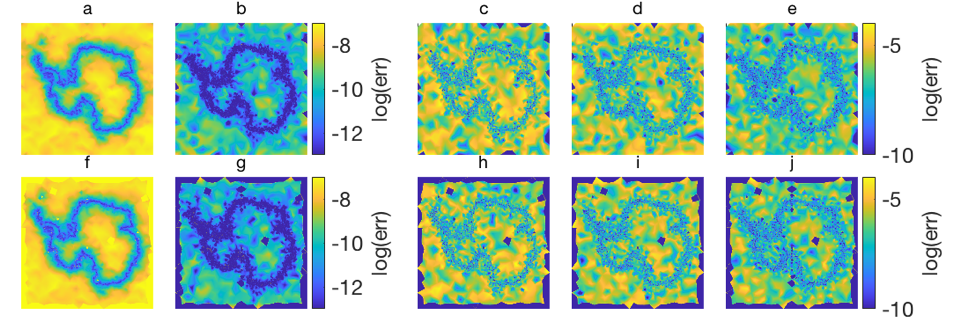
\includegraphics[width=0.9\linewidth]{Fig_discretisation_convergence_maps.png}
  \caption{Panels a-e: discretisation errors for the averaged-gradients approach used in UFEMISM for, from left to right, $f_x$, $f_y$, $f_{xx}$, $f_{xy}$ and $f_{yy}$. Panels f-j: the same for the least-squares approach from Syrakos et al. (2017).}
\end{figure}

To determine the order of convergence, discretisation errors are plotted against mesh resolution in \ref{fig:disc_conv_order}, with the panels ordered the same as in \ref{fig:disc_conv_maps}. Again, the results for both discretisation methods are virtually identical, with both showing a clear second-order convergence for the first-order partial derivatives, and first-order convergence for the second-order partial derivatives.

\begin{figure}[h!] \label{fig:disc_conv_order}
  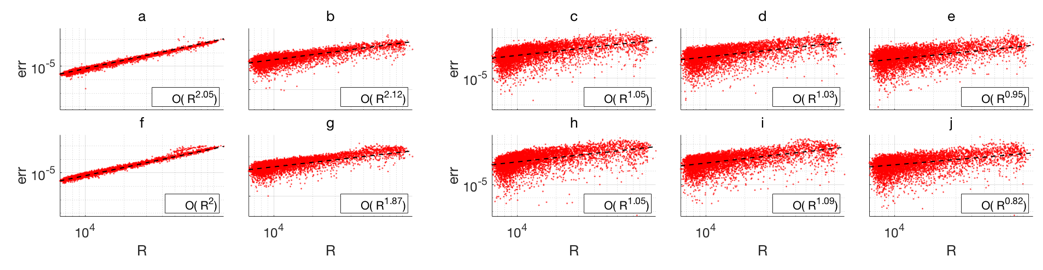
\includegraphics[width=0.9\linewidth]{Fig_discretisation_convergence_order.png}
  \caption{Panels a-e: discretisation errors vs. mesh resolution for the averaged-gradients approach used in UFEMISM for, from left to right, $f_x$, $f_y$, $f_{xx}$, $f_{xy}$ and $f_{yy}$. Panels f-j: the same for the least-squares approach from Syrakos et al. (2017). Logarithmic fits have been made for all graphs, with the order of convergence shown in the labels.}
\end{figure}


\subsection{Remapping}

\subsubsection{Theory}

Whenever UFEMISM updates the mesh, (some of) the model data must be remapped from the old to the new mesh. Extensive preliminary experiments have shown that the his to be done using a conservative remapping scheme. If, for example, simpler schemes like nearest-neighbour, linear, quadratic, or even cubic interpolation are used, significant errors show up in the results of the schematic benchmark experiments. In the Halfar experiment, the ice thickness tends to "flatten out". In the EISMINT experiment, the basal temperature at the ice divide shows a significant warm bias. All of these anomalies disappear when a conservative remapping scheme is used. The conservative remapping scheme developed for UFEMISM is based on the work of Jones (1999). The mathematical principles behind this approach are quite straightforward, but creating an implementation that is both robust and fast enough to handle meshes of hundreds of thousands of vertices was surprisingly difficult.

Let there exist two meshes that both cover the same domain: a "source" mesh (indicated henceforth by the subscript $s$) and a "destination" mesh (subscript $d$). Suppose the source mesh is the one that existed before a mesh update, and the destination mesh is the newly generated mesh, so that we want to find a way to remap a data field $f_s$ from the source mesh to the destination mesh. In the conservative remapping approach proposed by Jones (1999), the values $f_d$ on the vertices of the destination mesh are found by integrating $f_s$ over the regions of overlap $A_{sd}$ between the Voronoi cells $A_s$ of the source mesh, and the Voronoi cells $A_d$ of the destination mesh:

\begin{equation} \label{eq:remap_sumint}
f_d = \frac{1}{|A_d|} \sum_s \iint_{A_{sd}} f_s dA.
\end{equation}

Since the Voronoi cells of a mesh generally are irregular polygons, these surface integrals are not very straightforward to solve. Instead, Jones (1999) uses the divergence theorem to convert the surface integrals $\int_{A_{sd}}$ over the region of overlap $A_{sd}$ into a line integral around the perimeter $C_{sd}$ of this region. However, Jones (1999), having an implementation in general circulation models in mind, derived his expressions in spherical coordinates. UFEMISM uses Cartesian coordinates, so the solution derived here will look slightly different.

In order to define the surface integral in \eqref{eq:remap_sumint}, the function $f_s$ is "undiscretised" using a simple first-order Taylor expansion:

\begin{equation} \label{eq:remap_Taylor}
f_s(x,y) = \overline{f_s} + {\left( \frac{\partial f}{\partial x} \right)}_s \left( x - x_s \right) + {\left( \frac{\partial f}{\partial y} \right)}_s \left( y - y_s \right).
\end{equation}

Here, $\textbf{r}_s = \left[ x_s, y_s \right]$ is the geometric centre of the Voronoi cell of vertex $s$ (which is generally not the same as the vertex itself!), and $\overline{f_s}$ is the discrete value of $f$ on source vertex $s$. Substituting \eqref{eq:remap_Taylor} into \eqref{eq:remap_sumint} yields:

\begin{align} \label{eq:remap_sumint2}
f_d &= \frac{1}{|A_d|} \sum_s \left[ \iint_{A_{sd}} dA \left( \overline{f_s} + 
{\left( \frac{\partial f}{\partial x} \right)}_s \left( x - x_s \right) + 
{\left( \frac{\partial f}{\partial y} \right)}_s \left( y - y_s \right) \right) dA \right] \\
&= \frac{1}{|A_d|} \sum_s \left[ \overline{f_s} \iint_{A_{sd}} + 
{\left( \frac{\partial f}{\partial x} \right)}_s \left( \iint_{A_{sd}} xdA - x_s |A_{sd}| \right) +
{\left( \frac{\partial f}{\partial y} \right)}_s \left( \iint_{A_{sd}} ydA - y_s |A_{sd}| \right) \right].
\end{align}

Using the divergence theorem, we rewrite the three remaining surface integrals as line integrals:

\begin{align} \label{eq:remap_lineints}
\iint_{A_{sd}} dA &= \oint_{C_{sd}} x dy, \\
\iint_{A_{sd}} x dA &= - \oint_{C_{sd}} xy dx, \\
\iint_{A_{sd}} y dA &= \oint_{C_{sd}} xy dy.
\end{align}

Substituting these into \eqref{eq:remap_sumint2} yields:

\begin{equation} \label{eq:remap_remap}
f_d = \sum_s \left[ w_0 \overline{f_s} + w_{1x} {\left( \frac{\partial f}{\partial x} \right) }_s + 
w_{1y} {\left( \frac{\partial f}{\partial x} \right) }_s \right].
\end{equation}

The three remapping weights $w_0$, $w_{1x}$, and $w_{1y}$ are defined as:

\begin{align} \label{eq:remap_weights}
w_0 &= \frac{1}{A_d} \oint_{C_{sd}} x dy, \\
w_{1x} &= \frac{-1}{A_d} \oint_{C_{sd}} xy dx, \\
w_{1y} &= \frac{1}{A_d} \oint_{C_{sd}} xy dy.
\end{align}

\subsubsection{Implementation}

The basic theory of conservative remapping described in the previous section is fairly straightforward. Creating an implementation that is both robust (being able to handle any possible combination of meshes, including the possibility of overlapping vertices or lines) and fast (being able to remap data between meshes counting tens of thousands of thousands of vertices without significantly slowing down the model) turned out to be a surprisingly difficult problem, which took almost three months of full-time work to solve.\\
\\
The main routines for remapping are \textsc{create\textunderscore remapping\textunderscore arrays\textunderscore conservative} (for creating the remapping weights, stored in the \textsc{type\textunderscore remapping\textunderscore conservative}) and \textsc{remap\textunderscore cons\textunderscore 2nd\textunderscore order\textunderscore 2d/3d} (for using them to remap a data field), which are located in the \textsc{mesh\textunderscore mapping\textunderscore module}. A basic program that uses these routines to remap some data fields between a source mesh \textsc{mesh\textunderscore src} and a destination mesh \textsc{mesh\textunderscore dst} looks like this:

\hrulefill
\begin{lstlisting}

PROGRAM remap_data_between_meshes

! Declare the source and destination meshes
TYPE(type_mesh) :: mesh_src
TYPE(type_mesh) :: mesh_dst
! Declare the original (source) and remapped (destination) data fields
REAL(dp), DIMENSION(:), POINTER :: d1_src, d2_src, d3_src
REAL(dp), DIMENSION(:), POINTER :: d1_dst, d2_dst, d3_dst
INTEGER :: wd1_src, wd2_src, wd3_src, wd1_dst, wd2_dst, wd3_dst
! Declare the remapping arrays
TYPE(type_remapping_conservative) :: map

! Create the two meshes
...

! Create the remapping arrays
CALL create_remapping_arrays_conservative( mesh_src, mesh_dst, map)

! Allocate memory for the data fields
CALL allocate_shared_dp_2D( mesh_src%nV, d1_src, wd1_src)
CALL allocate_shared_dp_2D( mesh_src%nV, d2_src, wd2_src)
CALL allocate_shared_dp_2D( mesh_src%nV, d3_src, wd3_src)
CALL allocate_shared_dp_2D( mesh_dst%nV, d1_dst, wd1_dst)
CALL allocate_shared_dp_2D( mesh_dst%nV, d2_dst, wd2_dst)
CALL allocate_shared_dp_2D( mesh_dst%nV, d3_dst, wd3_dst)

! Remap the data
CALL remap_cons_2nd_order_2D( mesh_src, mesh_dst, map, d1_src, d1_dst)
CALL remap_cons_2nd_order_2D( mesh_src, mesh_dst, map, d2_src, d2_dst)
CALL remap_cons_2nd_order_2D( mesh_src, mesh_dst, map, d3_src, d3_dst)

END PROGRAM remap_data_between_meshes

\end{lstlisting}
\hrulefill
\\
\\
In the previous section, we showed that the values of $f$ on the vertices of the destination mesh consist of linear combinations of the values of $f$ on the vertices of the source mesh. As with the neighbour functions, we can calculate the linear coefficients (i.e. the remapping weights in eqs. \eqref{eq:remap_weights}) once for a pair of meshes, then apply them to any and all data fields that need to be remapped. These remapping weights are expressed using line integrals around the perimeter $C_{sd}$ of the area of overlap $A_{sd}$ between the Voronoi cells of source vertex $s$ and destination vertex $d$. Since the perimeter $C_{sd}$ is made up of subsets of the perimeters of the two Voronoi cells, we can therefore calculate the line integrals around the Voronoi cells of all vertices of both meshes, keeping track of the Voronoi cells of the opposite mesh through which they pass. The results of these two calculations can then be combined to give the line integrals around each of the areas of overlap, which will then be used to give the remapping weights defined in \eqref{eq:remap_weights}.\\
\\
Consider the (zoomed-in selections of) two meshes in \ref{fig:remapping}, panels A and C. The Voronoi cells of these meshes are shown in panels B and D, respectively.

\begin{figure}[H] \label{fig:remapping}
  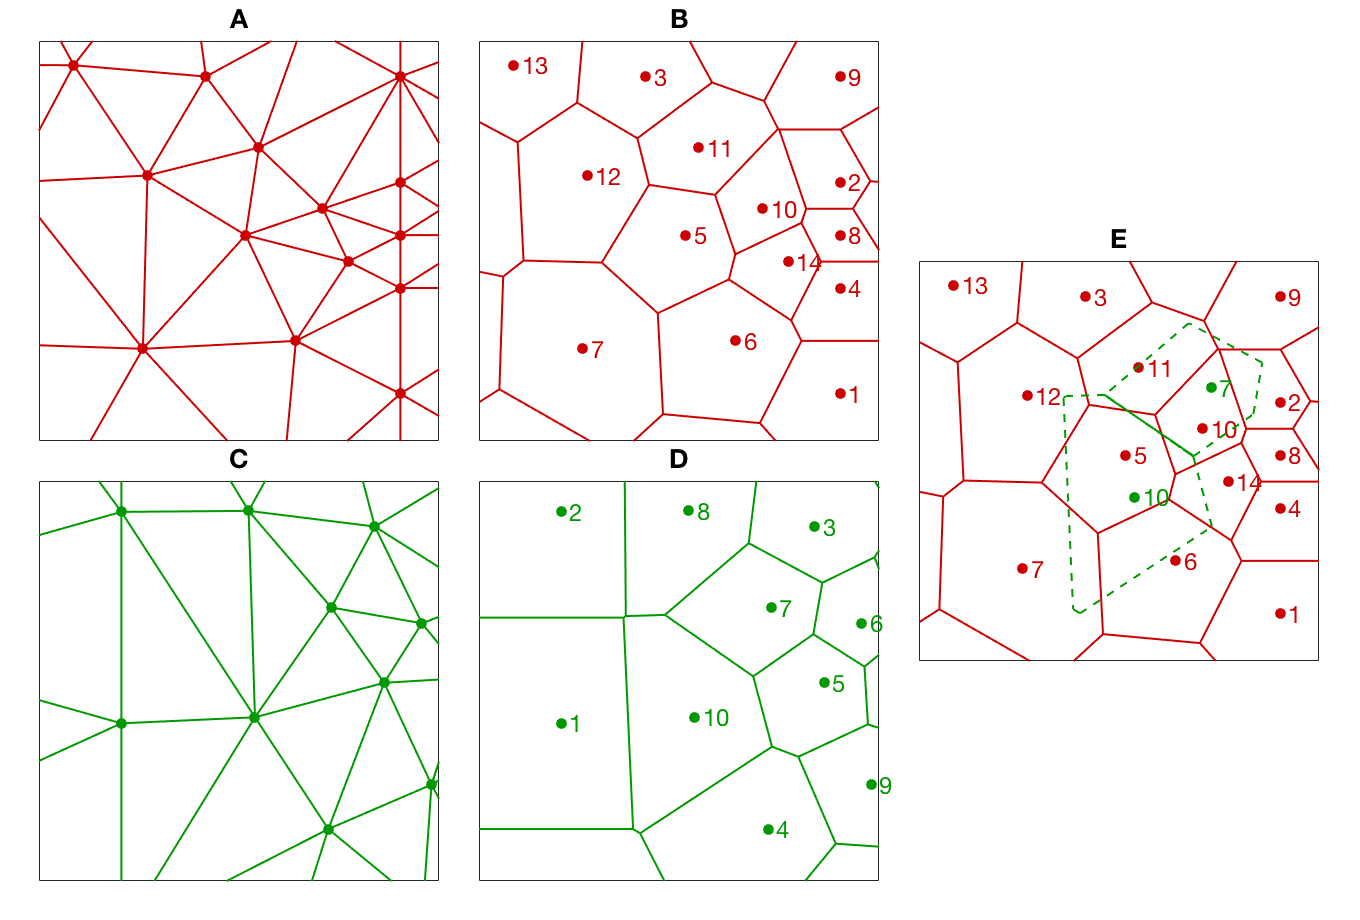
\includegraphics[width=0.9\linewidth]{Fig_remapping.png}
  \caption{A) the source mesh, B) the Voronoi cells of the source mesh, C) the destination mesh, D) the Voronoi cells of the destination mesh, E) two Voronoi cells of the destination mesh overlaid on the source mesh}
\end{figure}

Suppose we want to calculate the three line integrals from \eqref{eq:remap_lineints} over the shared boundary between the Voronoi cells of destination (green) mesh vertices 7 and 10, shown by the solid green line in \ref{fig:remapping}, panel E. This line passes through the source (red) mesh Voronoi cells of vertices 10, 5 and 11. In order to integrate over all the individual areas of overlap, the line integrals must be calculated over the three subsections of this line, and the results stored separately, recording the indices of both the source and destination vertices, lying on both the left-hand and right-hand sides of the line subsections. For this particular line, the results look like this:

\begin{center}
\begin{tabular}{ | m{5em} | m{5em} | m{5em} | m{5em} | m{5em} | m{5em} | m{5em} | } 
\hline
Left-hand source vertex & Right-hand source vertex & Left-hand destination vertex & Right-hand destination vertex & $\int xdy$ & $\int xydx$ & $\int xydy$ \\
\hline
10 & 10 & 10 & 7 & \ldots & \ldots & \ldots \\
5 & 5 & 10 & 7 & \ldots & \ldots & \ldots \\
11 & 11 & 10 & 7 & \ldots & \ldots & \ldots \\
\hline
\end{tabular}
\end{center}

The number of Voronoi cells of the opposite mesh through which a line passes is not generally known in advance. Finding the results shown above therefore requires an iterative algorithm which ''traces'' a line through a mesh; starting at one of the endpoints of a line, it will find the first point along the line where it crosses a Voronoi cell boundary of the mesh. The section of the line between the endpoint and the crossing point is integrated over, and is removed from the line, so that the crossing point now becomes the new end point. This is repeated until the entire line has been integrated over.\\
\\
For the three sections of this particular line, the left-hand and right-hand source vertex indices are the same. This is not the case when Voronoi cell boundaries of the two meshes coincide – something that, due to the deterministic nature of Ruppert’s algorithm, occurs quite frequently in UFEMISM. If the line integrals over coinciding line sections are calculated for both meshes, they will be double-counted when calculating the closed loop integrals, and the resulting surface integral will be incorrect. To prevent this, a flag must be raised when a coincidence is detected. When this is the case, only one of the two meshes is allowed to calculated the line integrals; the other one will simply list zero.\\
\\
The subroutine \textsc{create\textunderscore remapping\textunderscore arrays\textunderscore conservative}, which calculates the remapping weights, is structured like this:
\hrulefill
\begin{lstlisting}

SUBROUTINE create_remapping_arrays_conservative

    ! Find the coordinates and relevant indices of the Voronoi boundary lines.
    CALL find_Voronoi_boundary_lines( mesh_src)
    CALL find_Voronoi_boundary_lines( mesh_dst)

    ! Integrate over all Voronoi cell boundary lines for both meshes
    CountCoincidences = .FALSE.  
    CALL integrate_over_Voronoi_boundaries( mesh_src, mesh_dst, CountCoincidences)
    CountCoincidences = .TRUE.  
    CALL integrate_over_Voronoi_boundaries( mesh_dst, mesh_src, CountCoincidences)

    ! Rearrange integral contributions from Aci to vertices
    CALL rearrange_contributions_from_lines_to_vertices( mesh_src)
    CALL rearrange_contributions_from_lines_to_vertices( mesh_dst)

    ! Integrate around domain boundary
    CALL integrate_around_domain_boundary( mesh_dst, mesh_src)

    ! Add contributions from mesh_src to mesh_dst
    CALL add_contributions_from_opposite_mesh( mesh_dst, mesh_src)

    ! Finish incomplete mesh_dst vertices
    CALL finish_incomplete_vertices( mesh_dst, mesh_src)

    ! Convert line integrals to remapping weights
    CALL calculate_remapping_weights_from_line_integrals( mesh_dst, mesh_src, map)
      
    ! Check if everything worked
    CALL check_if_remapping_is_conservative( mesh_src, mesh_dst, map)

END SUBROUTINE create_remapping_arrays_conservative

\end{lstlisting}
\hrulefill
\\
\\
The different subroutines called here perform the following operations:
\begin{itemize}
\item \textsc{find\textunderscore voronoi\textunderscore boundary\textunderscore lines}: First, the coordinates of the endpoints of all the line segments constituting the Voronoi cell boundaries are determined for both meshes. Most of the time these are simply the circumcentres of the triangles of the mesh; the only exceptions occur for the Voronoi cells of vertices lying on the domain boundary.
\item \textsc{integrate\textunderscore over\textunderscore voronoi\textunderscore boundaries}: Then, the line integrals over all subsections of these line segments are calculated, as illustrated in Fig. \ref{fig:remapping}. It is possible that a Voronoi cell boundary of \textsc{mesh\textunderscore src} will (partly) coincide with one of \textsc{mesh\textunderscore dst}. In that case, that line must be integrated over only once, to prevent double-counting. The line-tracing algorithm that is used by \textsc{integrate\textunderscore over\textunderscore voronoi\textunderscore boundaries} can detect such coincidences; if the flag \textsc{countcoindidences} is set to \textsc{false}, the line integral over that segment will be listed as zero.
\item \textsc{rearrange\textunderscore contributions\textunderscore from\textunderscore lines\textunderscore to\textunderscore vertices}: Once the line integrals have been calculated, they are stored ''per line''. However, we want to have them available per vertex, so that they can be added together to give the loop integrals in Eqs. \eqref{eq:remap_weights}. This rearrangement step is done here.
\item \textsc{integrate\textunderscore around\textunderscore domain\textunderscore boundary}: Since the Voronoi boundaries were defined using staggered vertices, the boundary sections lying on the domain boundary are not included. These are treated separately by this subroutine.
\item \textsc{add\textunderscore contributions\textunderscore from\textunderscore opposite\textunderscore mesh}: The perimeter of a region of overlap between Voronoi cells of \textsc{mesh\textunderscore src} and \textsc{mesh\textunderscore dst} is made up of Voronoi cell boundaries of both meshes. In order to calculate the loop integral, the line integral sections from both meshes must be combined, which is done in this subroutine.
\item \textsc{finish\textunderscore incomplete\textunderscore vertices}: Sometimes the Voronoi cell of a \textsc{mesh\textunderscore dst} vertex will be completely enclosed by that of a \textsc{mesh\textunderscore src} vertex, or vice versa. These relatively rare exceptions are handled separately by this routine.
\item \textsc{calculate\textunderscore remapping\textunderscore weights\textunderscore from\textunderscore line\textunderscore integrals}: In this last step, the loop integrals are filed into \eqref{eq:remap_weights} to calculate the remapping weights.
\item \textsc{check\textunderscore if\textunderscore remapping\textunderscore is\textunderscore conservative}: To make sure everything works as intended, the remapping weights are applied to a dummy data field. On very rare occasions (estimated 1 in 100,000 vertices), minor errors occur when a vertex of one mesh lies exactly on the Voronoi cell boundary of a vertex of the other mesh. These erroneous vertices are detected by this routine, and their remapping weights are replaced by those representing simple bilinear interpolation.
\end{itemize}


\newpage
\section{Personal note}

By Tijn Berends, February 2021.\\
\\
In early 2019, the last year of my PhD at IMAU, I found myself with some spare time, sitting around and waiting for some particularly long ANICE simulations to finish (simulating the Lake Agassiz outburst flood during the last deglaciation, I believe). For some reason, the idea popped into my head that I should write a little Matlab program to create an unstructured grid. Not unusual for me - over the course of my PhD I wrote three different multi-purpose plotting programs, two text adventures, and a program for making 3D-printed ice sheets (I still have one lying on my desk!), all with the excuse of ''my model's running!''. Got to do something to keep the brain gears from rusting.\\
\\
The first few attempts didn't look like much, but after a day or two I figured out a nice way to describe a triangular grid data-wise. A quick internet search and some late nights spent drawing triangles on paper got me to write out a very basic refinement scheme. By then the idea that I'd use this as the basis for a new ice-sheet model had already crept up on me. It just seemed so very elegant; triangles can fit together any way you want them to, so you can make them small or large wherever you please. The benefits of this seemed obvious to me, though I hadn't yet started digging into the literature on grounding-line migration or other resolution-related issues. Creating a proper algorithm for mesh adaptation and writing out the discretisation of the model equations took me almost half a year. Around July I had a version that could solve the SIA, but creating a solution for the SSA took until early December. At that point I had a model that could do basic simulations of the Antarctic ice sheet; reading in input data for geometry and climate, calculating a mass balance, solving the ice dynamics, and updating the mesh whenever the ice geometry changed.\\
\\
So, in January 2020 I put together a few nice, sleek-looking animations and went to visit Roderik (then my promotor, now still my supervisor). ''Do you have a moment for me somewhere this week? I have something nice to show you.'', I mailed late on Sunday evening. Not ten minutes later came the reply: ''If it's really nice I have time first thing tomorrow morning.'' So, on Monday morning I spent just over an hour describing my pet project to Roderik. He asked a handful of questions throughout, otherwise just leaning back and observing. When I was finished, he was quiet for a moment, and he said to me, ''Well, I think it's interesting.''. He's not a very wordy man. However, early the next day he came to my office again, together with Heiko (Goelzer, then a postdoc at IMAU). ''Show him what you showed me'', Roderik told me. So I did. The two of them were very enthusiastic this time, and we agreed that I should finish up what I had into a paper, and they'd see if they could find a good way to put it to use. A few weeks later, on 31 January 2020, I defended my PhD thesis. In the laudatio, Roderik stated that the most memorable moment of my PhD happened at the very end of it when, ''having already finished the thesis, one day Tijn showed up and said he had something nice to show me - and I nearly fell from my chair with amazement!''. Not exactly how I remember it going, but I'll take it.\\
\\
In May 2020 we wrote and submitted (I wrote, Roderik submitted) a proposal to NWO, asking them to fund a project to finish develop UFEMISM and apply it to some nice palaeoglaciological research. While initially the plan was to use the funding (if we got it) to hire myself for a three-year postdoc, another position opened just after we'd submitted the proposal. Rather than gamble on a proposal that would take another 8 months at least to be processed, I decided to take the other position instead, and use the funding (if we got it) to hire someone else to carry out my ideas. Just over a week ago (early Feburary 2021) we received word that the proposal was accepted, and so it's now confirmed that UFEMISM will be, as they say, a thing. Where before I'd kept only some very basic ''documentation'' just for myself, I've now set myself to the task of writing out a complete description of everything I've created. That will be the rest of this document; this final page right here I wrote simply to please my own ego. Both the paper and the documentation are, as is tradition, phrased as ''we developed'', ''we chose'', ''we, we, we'', and I wanted to have just a little bit all to myself. Sue me.


\newpage
\section{References}

Berends, C. J., de Boer, B., and van de Wal, R. S. W.: Application of HadCM3@Bristolv1.0 simulations of paleoclimate as forcing for an ice-sheet model, ANICE2.1: set-up and benchmark experiments, Geoscientific Model Development 11, 4657-4675, 2018\\
\\
Berends, C. J., de Boer, B., Dolan, A. M., Hill, D. J., and van de Wal, R. S. W.: Modelling ice sheet evolution and atmospheric CO2 during the Late Pliocene, Climate of the Past 15, 1603-1619, 2019\\
\\
Berends, C. J., de Boer, B., and van de Wal, R. S. W.: Reconstructing the evolution of ice sheets, sea level, and atmospheric CO2 during the past 3.6 million years, Climate of the Past 17, 361-377, 2021\\
\\
Bintanja, R., van de Wal, R. S. W., and Oerlemans, J.: Global ice volume variations through the last glacial cycle simulated by a 3-D ice-dynamical model, Quaternary International 95-96, 11-23, 2002\
\\
Bueler, E. and Brown, J.: Shallow shelf approximation as a "sliding law" in a thermomechanically coupled ice sheet model, Journal of Geophysical Research 114, 200\\
\\
Determann, J.: Numerical modelling of ice shelf dynamics, Antarctic Science 3, 187-195, 1991\\
\\
Fettweis, X., Hofer, S., Krebs-Kanzow, U., Amory, C., Aoki, T., Berends, C. J., Born, A., Box, J. E., Delhasse, A., Fujita, K., Gierz, P., Goelzer, H., Hanna, E., Hashimoto, A., Huybrechts, P., Kapsch, M.-L., King, M. D., Kittel, C., Lang, C., Langen, P. L., Lenaerts, J. T. M., Liston, G. E., Lohmann, G., Mernild, S. H., Mikolajewicz, U., Modali, K., Mottram, R. H., Niwano, M., Noël, B. P. Y., Ryan, J. C., Smith, A., Streffing, J., Tedesco, M., van de Berg, W. J., van den Broeke, M. R., van de Wal, R. S. W., van Kampenhout, L., Wilton, D., Wouters, B., Ziemen, F., and Zolles, T.: GrSMBMIP: intercomparison of the modelled 1980-2012 surface mass balance over the Greenland Ice Sheet, The Cryosphere 14, 2020\\
\\
Greve, R.: Application of a Polythermal Three-Dimensional Ice Sheet Model to the Greenland Ice Sheet: Response to Steady-State and Transient Climate Scenarios, Journal of Climate 10, 901-918, 1997\\
\\
Huybrechts, P.: The Antarctic ice sheet and environmental change: a three-dimensional modelling study, Berichte zur Polarforschung 99, 1992\\
\\
Huybrechts, P. and de Wolde, J.: The Dynamic Response of the Greenland and Antarctic Ice Sheets to Multiple-Century Climatic Warming, Journal of Climate, 12, 2169–2188, 1999\\
\\
Janssens, I. and Huybrechts, P.: The treatment of meltwater re- tention in mass-balance parameterizations of the Greenland ice sheet, Ann. Glaciol., 31, 133–140, 2000\\
\\
Jones, P. W.: First- and Second-Order Conservative Remapping Schemes for Grids in Spherical Coordinates, Monthly Weather Review 127, 2204-2210, 1999\\
\\
Laskar, J., Robutel, P., Gastineau, M., Correia, A. C. M., and Levrard, B.: A long-term numerical solution for the insolation quantities of the Earth, Astronomy and Astrophysics 428, 261-285, 2004\\
\\
MacAyeal, D. R.: Large-Scale Ice Flow Over a Viscous Basal Sediment: Theory and Application to Ice Stream B, Antarctica, Journal of Geophysical Research 94, 4071-4087, 1989\\
\\
Martin, M. A., Winkelmann, R., Haseloff, M., Albrecht, T., Bueler, E., Khroulev, C., and Levermann, A.: The Potsdam Parallel Ice Sheet Model (PISM-PIK) - Part 2: Dynamic equilibrium simulation of the Antarctic ice sheet, The Cryosphere 5, 727-740, 2011\\
\\
Ohmura, A.: Precipitation, accumulation and mass balance of the Greenland ice sheet, Zeitschrift fur Gletscherkunde und Glazialgeologie, 35, 1–20, 1999\\
\\
Pollard, D. and DeConto, R. M.: Modelling West Antarctic ice sheet growth and collapse through the past five million years, Nature 458, 329-332, 2009\\
\\
Pollard, D.: A retrospective look at coupled ice sheet-climate modeiing, Climatic Change 100, 173-194, 2010\\
\\
Roe, G. H.: Modeling precipitation over ice sheets: an assessment using Greenland, Journal of Glaciology 48, 70-80, 2002\\
\\
Roe, G. H. and Lindzen, R. S.: The Mutual Interaction between Continental-Scale Ice Sheets and Atmospheric Stationary Waves, Journal of Climate 14, 1450-1465, 2001\\
\\
Ruppert, J.: A Delaunay Refinement Algorithm for Quality 2-Dimensional Mesh Generation, Journal of Algorithms 18, 548-585, 1995\\
\\
Singarayer, J. S. and Valdes, P. J.: High-latitude climate sensitivity to ice-sheet forcing over the last 120 kyr, Quaternary Science Reviews 29, 43-55, 2010\\
\\
Syrakos, A., Varchanis, S., Dimakopoulos, Y., Goulas, A., and Tsamopoulos, J.: A critical analysis of some popular methods for the discretisation of the gradient operator in finite volume methods, Physics of Fluids 29, 2017\\
\\
Weis, M., Greve, R., and Hutter, K.: Theory of shallow ice shelves, Continuum Mechanics and Thermodynamics 11, 15-50, 1999\\
\\
Winkelmann, R., Martin, M. A., Haseloff, M., Albrecht, T., Bueler, E., Khroulev, C., and Levermann, A.: The Potsdam Parallel Ice Sheet Model (PISM-PIK) - Part 1: Model description, The Cryosphere 5, 715-726, 2011\\
\\

\end{document}
